\documentclass[nonblindrev, copyedit]{informs3a}
%\documentclass[msom, nonblindrev, copyedit]{informs3a}

%\OneAndAHalfSpacedXI

\usepackage{endnotes}
\usepackage{enumerate}
\usepackage{color}
\usepackage{upgreek}
\usepackage{mathtools}
\usepackage{setspace, graphicx, booktabs, color, url, multirow}
\usepackage{siunitx}
\usepackage{booktabs}
\usepackage{amsmath}
\usepackage{amssymb}
\usepackage{graphicx}
\usepackage{textcomp}
\usepackage{makecell}
\usepackage{dsfont}
\usepackage{authblk}
\usepackage{blindtext}
\let\counterwithout\relax
\let\counterwithin\relax
\usepackage{chngcntr}
\usepackage{float}
\usepackage{url}
\usepackage{soul} % for highlight text
%\let\footnote=\endnote
\usepackage[dvipsnames]{xcolor}


\long\def\mh#1{{\color{cyan}#1}}
\long\def\jc#1{{\color{red}#1}}
\long\def\td#1{{\color{ForestGreen}#1}}
\long\def\que#1{{\color{orange}#1}}
\long\def\re#1{{\color{blue}#1}}
\newcommand\nc[1]{\textcolor{red}{NC: #1}}
\newcommand\cz[1]{\textcolor{blue}{CZ: #1}}


%\let\proof\relax
%\let\endproof\relax
%\let\theoremstyle\relax
%\usepackage{amsthm} % for proof
%\theoremstyle{definition}
%\newtheorem{definition}{Definition}[section]
%\theoremstyle{remark}

\definecolor{DarkBlue}{rgb}{0,0.08,0.45}
\usepackage[backref = false, bookmarks, breaklinks=true, colorlinks = true, plainpages = false, citecolor = DarkBlue, urlcolor = DarkBlue, filecolor = DarkBlue, linkcolor = DarkBlue]{hyperref}
\usepackage{natbib}
\let\oldbibliography\thebibliography
\renewcommand{\thebibliography}[1]{%
  \oldbibliography{#1}%
  \setlength{\itemsep}{-2.5pt}%
} % Reduce line space in References
\usepackage{float}
 \bibpunct[, ]{(}{)}{,}{a}{}{,}%
 \def\bibfont{\small}%
 \def\bibsep{\smallskipamount}%
 \def\bibhang{24pt}%
 \def\newblock{\ }%
 \def\BIBand{and}%
 \newcommand{\vp}{\vec{p}}
 \newcommand{\vq}{\vec{q}}
 \newcommand{\vy}{\vec{y}}
 \newcommand{\vz}{\vec{z}}
 \newcommand{\vx}{\vec{x}}
 \newcommand{\vd}{\vec{d}}
 \newcommand{\vu}{\vec{u}}
 \newcommand{\vZ}{\vec{Z}}
 \newcommand{\vI}{\vec{I}}
 \newcommand{\cQ}{\mathcal{Q}}
 \newcommand{\cY}{\mathcal{Y}}
 \newcommand{\cZ}{\mathcal{Z}}
 \newcommand{\cR}{\mathbb{R}}
 \newcommand{\cU}{\mathcal{U}}
 %\newcommand{\si}{\mathcal{S}}
 \newcommand{\eeps}{\boldsymbol{\epsilon}}
 \newcommand{\balpha}{\boldsymbol{\alpha}}
 \newcommand{\bbeta}{\boldsymbol{\beta}}
 \newcommand{\pe}{{E}}
 \newcommand{\ep}{\epsilon}
 \newcommand{\vr}{\vec{r}}
 \newcommand{\vzero}{\vec{0}}
 \newcommand{\lam}{\lambda}
 \newcommand{\bean}{\begin{eqnarray*}}
 \newcommand{\eean}{\end{eqnarray*}}
 \newcommand{\bea}{\begin{eqnarray}}
 \newcommand{\eea}{\end{eqnarray}}
 \newcommand\shline{
 \noalign{\global\savewidth\arrayrulewidth\global\arrayrulewidth 1.2pt}%
 \hline
 \noalign{\global\arrayrulewidth\savewidth}}
 \newcommand{\tabincell}[2]{\begin{tabular}{@{}#1@{}}#2\end{tabular}}

\newcounter{prop}[chapter]
\renewcommand*{\theprop}{\thechapter.\arabic{prop}}

\newenvironment{prop}{%
  \refstepcounter{prop}%
  \paragraph{Proposition~\theprop}%
  \renewcommand*{\theenumi}{\theprop\,(\roman{enumi})}%
  \renewcommand*{\labelenumi}{(\roman{enumi})}%
  \enumerate
}{%
  \endenumerate
}



 %\bibliographystyle{informs2014trsc}
\TheoremsNumberedThrough % Preferred (Theorem 1, Lemma 1, Theorem 2)
\ECRepeatTheorems
\EquationsNumberedThrough % Default: (1), (2), ...
\MANUSCRIPTNO{}

%%%%%%%%%%%%%%%%%%%%%%%%%%%%%%%%%%%%%%%%%%%%%%%%%%%%%%%%%%%%%%%%%%%%%%%%%%%%%%%%%%%%%%%%%%%%%%%%%%%%%%%%

\begin{document}
% Author's names for the running heads
\RUNAUTHOR{Chen et al.}

% Title or shortened title suitable for running heads.
\RUNTITLE{Capacitated SIR Model}

% Full title.
\TITLE{Capacitated SIR Model\\ with an Application to COVID-19}

\ARTICLEAUTHORS{
\AUTHOR{Ningyuan Chen, Ming Hu, Chaoyu Zhang}
\AFF{Rotman School of Management, University of Toronto, Toronto, Ontario M5S 3E6, Canada\\
\EMAIL{(ningyuan.chen, ming.hu, cyu.zhang)@rotman.utoronto.ca}}
%\AUTHOR{Ming Hu}
	%\AFF{Rotman School of Management, University of Toronto, Toronto, Ontario M5S 3E6, Canada,
	%\EMAIL{ming.hu@rotman.utoronto.ca}}
%\AUTHOR{Chaoyu Zhang}
	%\AFF{Rotman School of Management, University of Toronto, Toronto, Ontario M5S 3E6, Canada,
	%\EMAIL{cyu.zhang@rotman.utoronto.ca}}
}

\ABSTRACT{
The classical SIR model and its variants have seen great success in understanding and predicting epidemics' spread. We extend the SIR model to incorporate the limited testing capacity, which is by far one of the most notable challenges in the current COVID-19 outbreak. Specifically, on the SIR model, we impose a testing capacity that is shared among the infected and uninfected people. In this capacitated SIR model, we show first- and second-order structural properties of two measures, the total infections (confirmed or not) and the cases of unconfirmed infections, with respect to the testing capacity, degree of testing the uninfected (or level of hospital panic run), incubation/testing turnaround time, and infection rate. In particular, we show the total number of infection cases is concavely decreasing in the testing capacity. The policies to increase the testing capacity and to reduce the infection rate can be substitutable or complementary, depending on the chosen measure. We use COVID-19 data to calibrate our model and point out its public policy implications.
}
%\KEYWORDS{}

\maketitle


%\bigskip{}
%\noindent\rule[0.5ex]{\linewidth}{1pt}

%%%%%%%%%%%%%%%%%%%%%%%%%%%%%%%%%%%%%%%%%%%%%%%%%%%%%%%%%%%%%%%%%%%%%%%%%%%%%%%%%%%%%%%%%%%%%%%%%%%%%%%%

\section{Introduction}
\label{Introduction}

As the COVID-19 pandemic rages worldwide in 2020, all countries are working diligently to find effective ways to control this epidemic.
As of September 1, 2020, COVID-19 has hit almost every country globally, with more than 25.4 million reported cases. Researchers have studied various mathematical models to understand the spread of the virus and its transmission pattern. Among them, the classical SIR model and its variants, such as SEIR, are arguably the most popular ones. However, insufficient testing capacity, which limits the transition from one state to another, has not been appropriately accounted for in those classical models. There is a growing consensus that testing is a critical step to contain the outbreak, and in many countries, the current testing capacity is still below the desired level which can successfully mitigate the spread of the virus (\citealt{collins2020is}).

We build on the classical SIR model (see, e.g., \citealt{anderson1992infectious}) and incorporate the constraint of testing capacity.
In particular, we consider a parsimonious compartmental model with three simplified states: $S$ (susceptible), $I$ (infected but not yet confirmed), and $C$ (confirmed).
The parameters associated with the progress between states include the infection rate $\beta$, the testing capacity $K$, and the proportion of the susceptible (resp., unconfirmed infected) that get tested, $\delta$ (resp., $\gamma$).
In a two-period model, we show five main structural properties with respect to each of the aforementioned parameters.
Then we extend the results to multiple periods with additional conditions.
We calibrate our model with the COVID-19 data from all states in the United States and demonstrate the predictive power of the model.


To the best of our knowledge, this study is one of the first to thoroughly examine the impact of insufficient testing capacity theoretically, which leads to critical policy implications.
\cz{We investigate two different measures, the number of infected but undetected people and the total number of infected cases. 
We show that in most cases, the above mentioned first- and second-order properties with respect to $K$, $\delta$, $\gamma$, $\beta$ hold for both measures.}
First, as expected, increasing the testing capacity can reduce the total number of infections over time.
Having said that, we show that only when the testing capacity is large enough, the marginal value of having more testing capacity can be amplifying.
This implies the critical importance of having a large number of testing kits, or using the group testing technique to significantly ``expand" testing capacity.
Second, given that the testing capacity may not be elastically adjusted, it is beneficial to limit the testing of virus-free people.
The limited capacity imposes a negative externality, which is termed as the squeeze effect: the higher the degree of testing virus-free people is, the less testing kits are available for those who are truly in need, leaving more infected cases undetected and leading to more widespread infections. The squeeze comes from the testing resources ``wasted" on virus-free people unintentionally, then resulting in less testing resources available for infected people.
This explains why the Centers for Disease Control and Prevention (CDC) discouraged the virus-free from getting tested in the initial phase of COVID-19 \citep{overview}, and also stresses the importance of contact tracing, which uses the testing resources more selectively.
Third, we show that shortening the testing turnaround time, the period between the test and the result being available, pays off, with the marginal effect more significant when the period is already long. Put differently, shortening the testing turnaround time has a diminishing return.
Fourth, it is well known that reducing the infection rate is one of the most effective ways to slow down the spread.
The measures that are taken by many societies, such as social distancing in public areas, mask-wearing, and self-isolation when feeling unwell, are all aimed at such a goal.
Our study suggests that the marginal value of reducing the infection rate is increasing in the initial phase of epidemics.
That is, when the infection rate is low, further reducing the infection rate has little impact.
For a wide-spread disease, the phenomenon is reversed.
As a result, a combination of stringent rules is disproportionally more effective than a few loosely enforced measures.
Finally, we study the interaction of policies that reduce the infection rate and increase testing capacities.
We find that they are complementary in helping suppress the number of infected but undetected cases.
Therefore, it is crucial to pair up both types of policies to prevent the second wave.
On the other hand, when focusing on the total number of infections, the policies are substitutable.
which is also is confirmed by numerical studies of a few other papers.
Our result suggests that the policy makers should take caution when allocating resources to certain policies, as their synergetic effects can be ambiguous.

%%%%%%%%%%%%%%%%%%%%%%%%%%%%%%%%%%%%%%%%%%%%%%%%%%%%%%%%%%%%%%%%%%%%%%%%%%%%%%%%%%%%%%%%%%%%%%%%%%%%%%%%

\section{Literature Review}
\label{Literature Review}
Mathematical modeling has been playing an essential role in the study of infectious diseases.
In particular, epidemiological models, especially compartmental models, have seen great success.
They help us better understand the transmission of the diseases and eventually lead to effective measures to stop the spread.
\citet{hethcote2000mathematics} provides an overview of the popular models in this area.
In the SIR model, one of the most well-known compartmental models,
people are divided into three compartments: $S$ (susceptible), $I$ (infected), and $R$ (recovered).
People in state $S$ can progress to state $I$ with a certain transition rate and then progress to state $R$ with a recovery rate.
Focusing on the specifics of the development of COVID-19, \citet{atkeson2020will} uses the SIR model to predict the number of the infectious population over the next 12-18 months in the United States.
In particular, the author estimates the number of infected cases and predicts the overwhelming of the medical system.
\citet{acemoglu2020optimal} propose a multi-group SIR model and show that adopting differentiated lockdown policies for various groups is optimal.
The SEIR model extends the SIR model by incorporating an additional compartment $E$ (exposed), which represents those who are already infected but do not spread the disease.
This feature fits COVID-19, which has an incubation period that could be as long as 14 days and has a median of 4--5 days from exposure to symptoms onset.
\citet{peng2020epidemic} calibrate the SEIR model to predict the end of COVID-19.
\citet{birge2020controlling} propose a spatial model to provide an optimal way for social planners to control the spread of disease while reducing the economic costs.
The planners can implement targeted closures in specific ``hubs'' in a city and allow normal economic activities elsewhere.
\citet{toda2020susceptible} calibrates the SIR model for COVID-19 and studies the effectiveness of mitigation policies such as social distancing.
See also \cite{alvarez2020simple} for similar models on COVID-19.
In contrast, we propose a simple compartmental model with transition constraints and focus on the impact of testing capacity on the control of the disease.

Two papers capture testing capacity in a compartmental model. \citet{berger2020seir} use a compartmental model with 13 states to understand how different policies affect disease control.
The testing rate may affect the transition between certain states, but is determined exogeneously by the policy and not shared among the uninfected and the infected.
The authors find that testing and quarantine policies are both effective, and increased testing capacity can lead to less stringent targeted quarantine measures.
\citet{housni2020can} propose a compartmental model with 13 states to study the effects of testing capacity and social distancing measures on the evolution of the pandemic.
Like ours, their model also allows the testing capacity to be shared by infected and uninfected people.
The authors show that the testing capacity must increase if New York City wants to relax the social distancing measures during reopening, which implies that the mitigation policies of testing capacity expansion and social distancing measures are substitutable.
Their model is very comprehensive and captures the major characteristics of COVID-19, including  the existence of asymptomatic cases, isolation, and hospitalization.
Instead, our model is more high-level and only tracks the testing phase of the cases, while we also model the different inclination the uninfected and the infected may have to get tested.
The simplification allows us to derive structural properties (e.g., on the testing capacity and the degree of testing virus-free people) and stably calibrate the model parameters from the data.
Moreover, we are able to show the substitutability of the two types of policies theoretically, for one of the measures we consider.
However, the relationship can be reversed for another measure.
It suggests the policy makers take extra caution when accounting for synergy of the policies.

%The key difference of our paper from the above two papers is that we focus on deriving first- and second-order monotonicity properties, which are not the usual focus of a compartmental model, while the above two papers aim at calibrating the model and performing counterfactual analysis.




The impact of insufficient testing on the spread of COVID-19 and candidate solutions have been studied in the literature.
\citet{salathe2020covid} argue that increasing the testing capacity is an important approach to controlling COVID-19 in Switzerland.
The authors compare the economic impacts between the strategies of ``more testing, contact tracing and self-isolation'' and ``social-distancing''.
In the short term, the economic cost of the former strategy may be high, while social distancing measures are less expensive.
In the long term, social distancing may considerably hinder economic development, and the former strategy involving the increase of testing capacity can slow down the pandemic more effectively.
Note that this paper does not quantify the exact impact of increasing testing capacity on controlling the COVID-19 pandemic.
%But this article did not use a mathematical model to verify the author's conclusion, he just gave some examples to compare the impact of different measures on the control of the epidemic.
\citet{gollier2020group} show the testing capacity for COVID-19 is a bottleneck in April 2020 and suggest group testing to facilitate the process.
Indeed, group testing is an effective way to solve the problem of insufficient testing kits, which can immediately ``expand" the testing capacity.
More recently, \citet{aprahamian2019optimal} investigate the designs of optimal risk-based Dorfman group testing schemes.
As far as we know, no studies have investigated the impact of testing capacity on the spread of COVID-19 theoretically.
\citet{Drakopoulos2020why} use an analytical model to demonstrate that moderately good but earlier launched tests can outperform perfect but late tests when the testing capacity is low.
In contrast, our paper uses a variant of the SIR model to show the effectiveness of increasing testing capacity as well as the sensitivity with respect to other parameters.
We then validate the model predictions using the COVID-19 data in the United States.




There are many other studies whose insights help the fight against COVID-19 in dimensions other than the ones mentioned above. For example,
\citet{kaplan2020covid} adopts a scratch model to provide some guidance on decision making at the local level. The advice includes crowd-size restrictions, timing decisions of reopening restaurants and schools, and hospital surge planning. \citet{piguillem2020optimal} show that random testing is a very close substitute of quarantine and can substantially reduce the need for indiscriminate quarantines.
In \citet{chen2020hospital}, the authors investigate the roles played by hospital admission and social distancing in the slowdown of the spread, when the medical capacity is limited.



Finally, the way we capture the limited capacity is similar to \citet{ho2002managing}. In a new-product diffusion setting, \citet{ho2002managing} generalize the celebrated Bass model (which is analogous to the SIR model) by allowing for a supply constraint and derive the optimal capacity and time-to-market policies. Their supply constraint is analogous to the testing capacity in our model.




\section{The Model}
\label{The Model}
In this section, we introduce the setup of our capacitated SIR model. We then focus on four main structural properties of our model and present how the model parameters affect the epidemic trajectory.
\subsection{Model Setup}
\label{Model Setup}

We consider a compartmental model of three states:
\begin{itemize}
    \item $S$: the susceptible population.
    \item $I$: the infected population. Those in this state are not tested and can potentially infect the susceptible population.
    \item $C$: the confirmed. After tested positive, those in this state stay in self-quarantine or are hospitalized, and therefore do not infect the susceptible.
\end{itemize}
Since we focus on the effect of testing capacity, for parsimony, our study does not incorporate the treatment/hospitalization phases, and we do not explicitly model the subsequent outcomes of the infected after they are tested positive. In the empirical study of COVID-19, we calibrate our model up to the data of confirmed cases and do not go further to the cases of death.
We normalize the size of the population to 1, i.e., $S+I+C=1$ holds at any time.

Next, we describe the transitions between the states.
We consider a discrete-time model and use subscript $t$ to index a period.
Given the state $(S_t, I_t, C_t)$ at $t$, in the next period $t+1$, a fraction of the susceptible $S_t$ are infected, which is proportional to the percentage of infected cases over the unquarantined population, i.e., the sum of $S_t$ and $I_t$.
In particular, we have
\begin{equation}\label{eq:S_t recursive equation}
S_{t+1}=(1- \beta \frac{ I_{t}}{S_{t}+I_{t}})S_{t}.
\end{equation}
Here, $\beta$ represents the expected number of people an infected person infects per period after proper normalization.
This is a standard setup in similar compartmental models.

For the infected population, other than the newly infected, some of them are tested positive and progress to state $C$.
Suppose there are $\delta S_t+\gamma I_t$ people intending to get tested in period $t$ in a testing facility, with a fraction $\delta$ of the healthy ($S_t$) and $\gamma$ of the infected ($I_t$).
The parameter $\delta$ reflects the degree of virus-free people being tested. In February 2020, at the epicenter of the pandemic, healthy people rushed to the local hospital of Wuhan to get examined. Hence, the parameter $\delta$ could also capture the level of public panic to run the healthcare resources.
The parameter $\gamma$ reflects the fact that the disease has an incubation period, and the testing result is not available immediately, both delaying the transition from state $I$ to state $C$.
We may approximate $\gamma$ by $\gamma=1/(\text{average incubation time}+\text{testing turnaround time})$: if it takes 5 days from the moment that a person gets infected to being confirmed positive and the system reaches a steady state, then on average 20\% of $I$ transits to $C$ each day.
With this interpretation,
we expect $\delta$ to be small relative to $\gamma$.
We also assume that the testing accuracy is $\eta$, which can be interpreted as one minus the false-negative rate.
The testing is subject to capacity $K_t$, which tends to be less than $\delta S_t+\gamma I_t$, due to the limited number of testing kits.
The rationing of limited capacity among those who want to participate in the testing is conducted in a purely random way.
Combining the factors mentioned above, we thus have the number of
infected cases being confirmed in period $t$ as:
\begin{equation*}
    \eta\min\left\{1,\frac{K_t}{\delta S_{t}+\gamma I_{t}}\right\}\gamma I_{t}.
\end{equation*}
We do not consider the false positive which can be effectively eliminated by independent and repeated testing.
As a result, the dynamics of $I_t$ and $C_t$ follow
\begin{align}
I_{t+1}&=\frac{\beta I_{t}}{S_{t}+I_{t}}S_{t}+\left(1-\eta\gamma \min\left\{1,\frac{K_t}{\delta S_{t}+\gamma I_{t}}\right\}\right)I_{t},\label{eq:I_t recursive equation}\\
C_{t+1}&=\eta\gamma\min\left\{1,\frac{K_t}{\delta S_{t}+\gamma I_{t}}\right\}I_{t}+C_{t}.\label{eq:C_t recursive equation}
\end{align}
%The dynamics and transitions are summarized in the following matrix:
%\begin{equation*}
%\left[ \begin{array}{cccc}
%1-\frac{\beta I}{S+I} & \frac{\beta %I}{S+I} & 0\\
%0 & 1-\eta\gamma \min\{1,\frac{K_t}{\delta S+\gamma I}\}& \eta\gamma \min\{1,\frac{K_t}{\delta S+\gamma I}\}\\
%0 & 0 & 1
%\end{array}
%\right ]
%\end{equation*}
%In the theoretical analysis, we assume $\eta=1$, which means that the testing kits are $100\%$ accurate.
%while we allow for $\eta<1$ the counterfactural analysis of our empirical study.
By definition, $\beta\ge 0$, $0<\delta\le 1$, $0<\gamma\le 1$, and $0<\eta\le 1$. Figure~\ref{fig:transition} illustrates the transition dynamics of our capacitated SIR model. Table~\ref{Table Estimated Parameters} provides a summary of our model parameters.

\begin{figure}[ht]
	\centering
 	\caption{Transitions between the states of the model}
 	\label{fig:transition}
	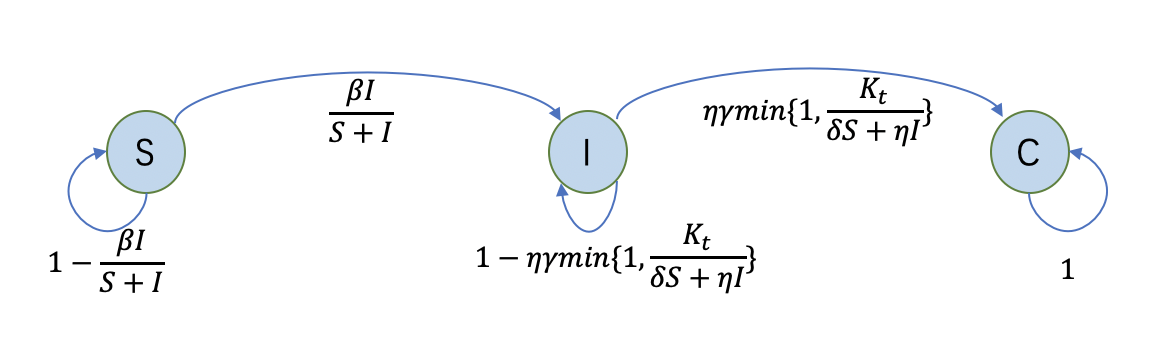
\includegraphics[width=0.8\linewidth, angle=0]{transition_fig.png}
\end{figure}


\begin{table}[ht]
	\centering
	\fontsize{9}{15}\selectfont
	\caption{A summary of model parameters}

	\label{Table Estimated Parameters}
	\setlength{\tabcolsep}{5mm}{
	\begin{tabular}{l l l l}
	\Xhline{2\arrayrulewidth}
	\tabincell{l}{Parameter} & \tabincell{l}{Interpretation} &  \tabincell{l}{Structural result on $I_2+C_2$} &
	\tabincell{l}{Policy implication} \\
	\Xhline{2\arrayrulewidth}
	$K$ & Testing capacity  & Increasing and concave & Testing capacity expansion \\
	\hline
	\tabincell{l}{$\delta$} & \tabincell{l}{Degree of testing the\\ uninfected and panic run } & \tabincell{l}{Increasing and concave} & \tabincell{l}{Contact tracing, and self-quarantine, \\stay at home unless severely ill} \\
	\hline
	\tabincell{l}{$\gamma$} & \tabincell{l}{Reciprocal of incubation\\ and testing turnaround time} & \tabincell{l}{Decreasing and convex} & \tabincell{l}{Testing turnaround time shortening} \\
	\hline
	\tabincell{l}{$\beta$} & \tabincell{l}{Infection rate} & \tabincell{l}{Increasing \\If $2S_1\ge S_0+I_1$, convex; \\otherwise, concave} & \tabincell{l}{Social distancing, mask-wearing,\\quarantine}\\

	\Xhline{2\arrayrulewidth}
	%\multicolumn{4}{p{15cm}}{\emph{Note:} Other parameters are set as follows: $\lambda=5$, $\gamma=0.5$, $L=5$, $c=0.5$, and $\theta=3$.} \\
	\end{tabular}}
\end{table}

\subsection{Structural Properties}
\label{Structural Properties}
Next, we derive a set of structural properties for our model.
We assume that $S_t>I_t$ holds for all $t$ and $\delta\le \gamma$, which correctly reflects the current situation as most people are uninfected and the healthy are less likely to get tested.
For ease of exposition, we assume that the testing kit is perfectly accurate, i.e., $\eta=1$. All results would hold for a constant $\eta<1$.
We also assume that $K_t= K$ and the testing is always capacitated. (In the empirical study, we allow the capacity to be time varying based on the collected data.)
The testing capacity as a bottleneck is particularly the case for COVID-19:
according to a U.S. News report \citep{Thompsan2020There}, testing supply is far below the demand, even by the end of July.

In period $t=0$, we have the initial states as:
\begin{align*}
S_0=s_0,\quad
I_0=1-s_0,\quad
C_0=0,
\end{align*}
where $0\le s_0\le1$. According to the system dynamics described earlier, at $t=1$ we have
\begin{align*}
S_1=D,\quad
I_1=1-D-\eta AK,\quad
C_1=\eta AK,
\end{align*}
where
\begin{align}\label{eq:AD-def}
   A\equiv\frac{\gamma(1-s_0)}{\gamma(1-s_0)+\delta s_0}\in[0,1],\quad D\equiv\beta s_0^2+(1-\beta)s_0\in [0,1].
\end{align}
At $t=2$, by \eqref{eq:S_t recursive equation} and \eqref{eq:I_t recursive equation}, we have
\begin{align*}
S_2&=D-\frac{\beta D(1-D-\eta AK)}{1-\eta AK},\\
I_2&=-\frac{K\gamma(1-D-\eta AK)}{\delta D+\gamma(1-D-\eta AK)}+1-D-\eta AK+\frac{\beta D(1-D-\eta AK)}{1-\eta AK}\\
&=-K+\frac{\delta DK}{\delta D+\gamma(1-D-\eta AK)}+1-D-\eta AK+\beta D-\frac{\beta D^2}{1-\eta AK},\\
C_2&=\eta AK+\frac{K\gamma(1-D-\eta AK)}{\delta D+\gamma(1-D-\eta AK)}.
\end{align*}
%For any $t\in\mathbb{N}$, we have
%\begin{align*}
%S_{t+1}&=S_{t}-\frac{\beta I_{t}S_{t}}{S_{t}+I_{t}},\\
%I_{t+1}&=\frac{\beta I_{t}S_{t}}{S_{t}+I_{t}}+I_{t}- \eta K\frac{\gamma I_{t}}{\delta S_{t}+\gamma I_{t}},\\
%C_{t+1}&=1-S_{t+1}-I_{t+1}.
%\end{align*}
In the main body of the paper, we show the structural properties in a two-period model, i.e., $t=2$. In the online appendix, we provide sufficient conditions for each of the structural properties to hold inductively for $t> 2$. After calibrating the model to the COVID-19 data in Section~\ref{sec:empirical}, we find that those properties largely hold throughout the whole observation window of several months.

For the structural properties, we focus on the following two measures $I_2+C_2$ and $I_2$.
The former one, $I_2+C_2$, represents the total number of infected people in period two, i.e., the number of infected but unconfirmed cases plus the number of infected and confirmed cases, which is arguably the measure of most interest. We assume that people in state $C$ as being confirmed are quarantined or hospitalized so that (1) humanitarianly, they have been taken care of, and (2) they are less likely to infect healthy people. \cz{On the other hand, the latter one, $I_2$, }is also a critical measure to be estimated because people in state $I$ are those who have been infected but not been detected yet, and thus they can potentially infect many others.
\cz{The measure $I_2$ is forward-looking, which is closely related to the diffusion of the disease in the near future, while the total number of infections ($I_2+C_2$) is an aggregated indicator of the current status of the disease's spread.
Our next result shows the impact of the testing capacity on these two measures.}
\begin{proposition}[{\sc Testing Capacity}]
\label{prop:with k}
\begin{enumerate}[(i)]
    \item\label{itm:first order with k} Both $I_2$ and $I_2+C_2$ are decreasing in $K$.
    \item\label{itm:i2c2 second order with k} $I_2+C_2$ is concave in $K$.
    \item\label{itm:i2 second order with k} If $\delta$ is sufficiently small, then $I_2$ is concave in $K$;\\ If $\delta$ is sufficiently close to $\gamma$, then $I_2$ is convex in $K$.
\end{enumerate}
\end{proposition}

Proposition \ref{prop:with k}\eqref{itm:first order with k} confirms that intuitively, with a higher testing capacity level, the number of unconfirmed cases of infection and the total number of infections decrease.
Proposition \ref{prop:with k}\eqref{itm:i2c2 second order with k} demonstrates that investing in the testing capacity has an increasing return on reducing the total number of infections.
That is, when the testing capacity is small, increasing the testing capacity has little value in the reduction of infections. Only when the testing capacity is sufficiently large does a marginal increase in $K$ have a significant value.
This result can be explained as follows: without testing and removing the infected from the population, additional testing capacity has little impact as the disease is still mostly out of control due to under-testing.
Only when the testing capacity is large enough can the spiral-down spread of disease be put under control.
This property underscores the importance of having a sufficiently large number of available testing kits.

Proposition \ref{prop:with k}\eqref{itm:i2 second order with k} shows that the marginal effect of testing capacity on the number of infected but unconfirmed cases depends on $\delta$, the degree of testing virus-free people. If the degree of testing virus-free people is small (or the panic run is not severe), the marginal benefit of having more testing kits on reducing the number of infected but unconfirmed people increases as more testing kits are available. This property is consistent with Proposition \ref{prop:with k}\eqref{itm:i2c2 second order with k}, when the testing capacity is not much wasted, which, again, points to the critical value of having a sufficiently high level of testing capacity. However, interestingly, if the proportion of testing virus-free people is close to the proportion of testing infected people (or the panic run is severe), the marginal benefit of having more testing kits on the number of infected but unconfirmed people decreases as more testing kits are available. 
In this case, due to the testing capacity proportionally ``wasted" on virus-free people, a marginal increase on a sufficiently small capacity level not only puts more infections under control but also, more critically, has a propagating effect of leaving fewer infections undetected and ``saving" more capacity for the infected in future periods.
%\cz{Although more testing capacity would proportionally allocated to infected people over time, this effect is dominated.}
As a result, when the testing is conducted close to a random fashion, the testing capacity has a diminishing return.



Proposition~\ref{prop:with k} has the following policy implications.
First, it is imperative to rack up the production scale of COVID-19 detection reagents quickly.
Second, it is acceptable to have relatively low testing accuracy in the early stage of the pandemic.
This is because only dramatically increasing the testing capacity can have a significant effect on reducing the total number of infections, in particular when the testing is targeted to the severely ill (i.e., $\delta$ is small).
Hence the impact of testing accuracy may be negligible if the testing capacity is low, and
inaccurate but abundant testing can do more good than harm \citep{Drakopoulos2020why}.
Third, technologies that can ``increase'' the testing capacity by maximizing its effectiveness without physically changing the capacity should be encouraged and adopted.
For example, group testing can be used to save the testing kits and improve testing efficiency.

\cz{Next, we investigate the impact of the degree of testing virus-free people on the two measures $I_2$ and $I_2+C_2$. We find that they have the same structural properties with respect to $\delta$.}

\begin{proposition}[{\sc Degree of Testing Virus-free People}]
\label{prop:with delta}
   \begin{enumerate}[(i)]
    \item\label{itm:first order with delta} Both $I_2$ and $I_2+C_2$ are increasing in $\delta$.
    \item\label{itm:second order with delta} Both $I_2$ and $I_2+C_2$ are concave in $\delta$.
   \end{enumerate}
\end{proposition}

Given that the testing capacity cannot be increased rapidly due to physical constraints, Proposition \ref{prop:with delta}\eqref{itm:first order with delta} shows that if we limit the number of tests potentially done to the virus-free people by more targeted testing, then the spread of the disease can slow down.
%number of unconfirmed cases of infection and total cases of infection will decrease.
Proposition \ref{prop:with delta}\eqref{itm:second order with delta} states that the marginal effect of reducing the fraction of virus-free people getting tested has a diminishing return.
That is, when there are few virus-free people get tested, reducing $\delta$ is more effective. However, when there is a panic run which can lead to more virus-free people getting tested, it is less effective to reduce the degree of testing virus-free people marginally, because the limited testing capacity tends to be already ``wasted" to a large extent and the undetected infections at one time will propagate to more infections in the future.

%\nc{We mentioned panic run in the intro but not here. We need to frame it consistently?}
Proposition \ref{prop:with delta} supports the conventional wisdom that we need to reserve the capacity of testing kits and other medical resources for those who truly need it.
This can be intuitively explained by the squeezing effect: the larger the proportion of testing virus-free people is, the less testing kits are available for real infected people, thus more infected people left unconfirmed.
To prevent the precious resources being ``wasted," it is reasonable to minimize the testing for those who do not have symptoms.
This is consistent with the latest CDC's guideline that people without COVID-19 symptoms are not encouraged to get tested (\citealt{Wu2020C.D.C.}). However, one negative example is, at the beginning of the pandemic in Wuhan, ``[p]anicked residents of the city are heading to the hospitals if they have any sign of a cold or cough'' (\citealt{wee2020what}). This panic run leads to a short supply in testing resources such as the testing kits. The lockdown policy could make it more difficult to get enough testing resources as needed.
%\nc{can we find support for how lockdown/reopen connects to $\delta$.}
Our result also implies that during the lockdown period, when the degree of testing virus-free people is relatively low, reducing the proportion of virus-free people get tested has a larger impact. But during the reopening period, when the degree of testing virus-free people is relatively high, reducing this proportion has little value.

\cz{Next, we show the impact of incubation and testing turnaround time on $I_2$ and $I_2+C_2$. Again, these two measures have the same structural properties with respect to the incubation/testing turnaround time.}
\begin{proposition}[{\sc Incubation and Testing Turnaround Time}]
\label{prop:with gamma}
    \begin{enumerate}[(i)]
    \item\label{itm:first order with gamma} Both $I_2$ and $I_2+C_2$ are decreasing in $\gamma$.
    \item\label{itm:second order with gamma} Both $I_2$ and $I_2+C_2$ are convex in $\gamma$.
   \end{enumerate}
\end{proposition}

Proposition~\ref{prop:with gamma}\eqref{itm:first order with gamma} demonstrates that if we can decrease the testing turnaround time (with a larger $\gamma$), then there will be less infected cases.
Proposition \ref{prop:with gamma}\eqref{itm:second order with gamma} implies that when the incubation and testing turnaround time is long (i.e., $\gamma$ is small), which is the case for the current pandemic of COVID-19, the marginal effect of reducing that time (equivalently, increasing $\gamma$) is more significant.
That is, intuitively, confirming the infected people by testing with a marginally faster pace has a diminishing return.
In fact, the problem of a long incubation period and testing turnaround time has received much attention.
\citet{popovich2020how} points out that the current average lag from symptom onset to positive tests is four days, which is longer than other infectious diseases.
\citet{Abbott2020CVS} report that customers complain about waiting for too long to receive the test result.
Our result implies that it is beneficial to shorten either time frame. Given both time frames are already long, any marginal decrease in those time frames would have a significant impact.

\cz{Moreover, we show the effect of infection rate on the total number of infected cases. 
The structural property of $I_2$, on the other hand, is quite challenging.
This is because $\beta$ only controls the process from state $S$ to $I$, while $I_2$ also largely depends on  the transition from $I$ to $C$.
Nevertheless, in the numerical experiments, we show that $I$ is convex in $\beta$ for the calibrated parameters.}
%Can we add a sentence on why there is no property on $I_2$.
%it is okay to say it's challenging. in addition, can we use some later numerical observations to give some insight on this $I_2$ w.r.t. beta numerically.

\begin{proposition}[{\sc Infection Rate}]
\label{prop:with beta}
    \begin{enumerate}[(i)]
    \item\label{itm:first order with beta} $I_2+C_2$ is increasing in $\beta$.
    \item\label{itm:second order with beta} If $2S_1\ge S_0+I_1$, then $I_2+C_2$ is convex in $\beta$. Otherwise, $I_2+C_2$ is concave in $\beta$.
   \end{enumerate}
\end{proposition}

Proposition \ref{prop:with beta}\eqref{itm:first order with beta} confirms that lowering the infection rate can effectively reduce the number of infections.
The marginal effect of such measures, as demonstrated by Proposition \ref{prop:with beta}\eqref{itm:second order with beta}, can be ambiguous.
If $2S_1\ge S_0+I_1$, then the marginal value of lowering the infection rate diminishes: when the infection rate is already low, its change has a smaller impact on the total number of infections.
This is typically the case in the initial phase of pandemics, in which we have $I_1\ll S_1$ and $S_1\approx S_0$.
A slight increase in the infection rate may drastically facilitate the spread and lead to much worse outcomes.
Therefore, it is crucial to keep the infection rate below a certain threshold, which leaves enough space and error tolerance for policy experimentation.
On the other hand, when $2S_1< S_0+I_1$, which is the case when a significant fraction of the population is infected (with a large infection rate), then it costs more to lower the infection rate and slow down the spread because of the decreasing marginal effect.
Although not explicitly modeled in this study, there have been a number of ways to reduce the infection rate, such as social distancing, mask-wearing, and quarantine.
For example, \citet{wu2020masks} reports that wearing masks can prevent people from spreading airway germs to others; in the meantime, masks can also protect people from being infected by others, which effectively reduce the infection in both ways.

\cz{Finally, we demonstrate the interaction of two commonly used policies, expanding testing capacity and quarantine/social distancing policies, on the two measures of $I_2$ and $I_2+C_2$.}

\begin{proposition}[{\sc Testing Capacity and Quarantine Policies}]
\label{prop:two policies}
    \begin{enumerate}[(i)]
    \item\label{itm:with i2}
    $I_2$ has increasing differences in $K$ and $-\beta$. 
    \item\label{itm:with i2c2} 
    If $\beta(1-s_0)\leq\frac{1}{2}$, then $I_2+C_2$ has decreasing differences in $K$ and $-\beta$. 
   \end{enumerate}
\end{proposition}

Proposition \ref{prop:two policies} studies the interactions between two types of commonly used policies: increasing testing capacity (increasing the testing capacity $K$) and quarantine/social distancing policies (decreasing the infection rate $\beta$). 
Proposition \ref{prop:two policies}\eqref{itm:with i2} shows that these two policies are complementary for reducing the number of infected but unconfirmed cases. Hence, for this goal, increasing the testing capacity and implementing quarantine policies at the same time are synergetic. That is, with one in action, the benefit of implementing the other increases.  
Interestingly, when we consider the impact of different policies on decreasing the total number of infected cases, this complementary relationship can be reversed. Proposition \ref{prop:two policies}\eqref{itm:with i2c2} states that when the infection rate or the existing infected cases is not extremely high, which is innocuous and seems to hold for almost all real life situations, increasing testing capacity and implementing quarantine policies are substitutable in reducing the total infected cases. That is, with one in action, the benefit of implementing the other is reduced. 
The reason why this result is reversed when we focus on the number of total infected cases is because the testing capacity $K$ mainly affects the process from state $I$ to state $C$. Thus, when we study the number of $I+C$, the effect of $K$ is less obvious and only shows up after a long period of time.
Proposition \ref{prop:two policies}\eqref{itm:with i2c2} also implies that when one action is already in play, the other may be relaxed, as the additional benefit of using both is limited. For example, when the testing capacity is insufficient, we can use more strict quarantine policies as compensations. On the other hand, if we plan to reopen and relax the social-distancing measures, the testing capacity must increase and more testing kits are needed.

Proposition \ref{prop:two policies} leads to a few recommendations for policy makers. 
Our results imply the interaction of various policies can be different depending on the measure under consideration. Recall that the number of infected but undetected cases is a more forward-looking measure, while the total number of current infections is more myopic (and the total number of death could be backward-looking). 
First, to control the spread of the disease, and prevent the second wave, it is imperative to suppress the number of infected but undetected cases ($I_2$).
Increasing the testing capacity should be paired with strict quarantine and social-distancing measures at the same time. 
Even with limited resources, the government should allocate them more or less evenly between the two categories.
For example, this strategy is adopted by South Korea, which pioneered the drive-through tests and ramped  up the testing capacity dramatically. 
Meanwhile, South Korea aggressively track the infected and quarantine their close contacts. 
In contrast, in the United States, little attention has been paid to quarantining the close contacts of people who were tested positive of COVID-19 \citep{Sharfstein2020testing}, which could an unending cycle of the number of infected cases going up and down.  
Second, focusing on the current total number of infected cases, the impact of reopening the economy, which would inevitably increase the infection rate, can be remedied by sufficient testing capacity.
%relaxing the social-distancing and quarantine policies by increasing the testing capacity for reopen and recovering economics. 
As shown in \citet{berger2020seir} and \citet{housni2020can}, the simulation results indicate that sufficient testing capacity can ``stand in'' for costly quarantine policies.
This view is adopted by most of the academic papers and policy makers. However, we caution that with the economy re-opened, the future infected cases would have a danger of shooting up leading to a possible second wave of the pandemic. 


\section{Empirical Study}\label{sec:empirical}
In this section, we calibrate our model's parameters by using the real COVID-19 data in the United States.
Based on the estimated parameters, we then conduct the counterfactual analysis by adjusting the testing capacity.
We also validate the structural properties of the model numerically.

\subsection{Data}
\label{Data}
We use the COVID-19 data from the COVID Tracking Project\footnote{\url{https://covidtracking.com/data}}.
This data source provides daily updates based on the information extracted from public health authorities and official statements of all states in the United States.
The dataset includes the daily number of completed viral tests and cumulative confirmed cases.
We note that many papers, such as \citet{toda2020susceptible} and \citet{birge2020controlling}, use alternative data sources such as the JHU data tracker\footnote{\url{https://coronavirus.jhu.edu/us-map}.} and New York Times Coronavirus data tracker\footnote{\url{https://www.nytimes.com/interactive/2020/us/coronavirus-us-cases.html}.}.
These datasets do not report the daily number of tests for a time period as long as the COVID Tracking Project, which is crucial to estimate our model.
In contrast, the COVID Tracking Project has complete testing data starting from the early March of 2020.

We normalize the population of each state, such that $S+I+C=1$.
The population data is obtained from the World Population Review\footnote{\url{https://worldpopulationreview.com/states/}.}.


When processing the data, we identify a few potential errors.
For example, the cumulative number of testing conducted may be decreasing over one day, possibly due to reporting or counting errors.
In such rare cases, we remove the days during which the daily testing number is negative.

\subsection{Estimation}
\label{Estimation}
We note that starting in March 2020, many states in the United States were locked down and stay-at-home orders were imposed to control the spread of the pandemic.
In May and June, many of them began to reopen.
According to the World Health Organization,
%the main way of COVID-19 spreads is through close contacts between individuals.
there is evidence that the lockdown can significantly change the behavior and slow down the spread of COVID-19.
%Stay-at-home can avoid close contacts with others and will protect people from possible COVID-19, thus make it harder for the spread of virus.
Therefore, it is reasonable to assume that the parameters belong to different regimes before and after lockdown/reopen. For example, one would expect that
%It is unreasonable to assume that the parameters such as $\beta$, $\gamma$ and $\delta$ would remain the same during different policy regimes.
during the lockdown, the infection rate $\beta$ becomes small, which contributes to the slowdown of the disease.

To incorporate the different policy regimes, we divide the data into three stages: Before Lockdown, Lockdown,  and Reopen. The exact date when each state started to lock down and reopen may differ across states and can be found in \citet{Elassar2020This}.
We estimate the parameters in each of the three stages separately.

We use the least-squares estimation for the parameters.
More precisely, we extract $K_t$ (the number of tests on day $t$) and $C_t$ (the daily number of confirmed cases) from the raw data by taking the difference of the respective cumulative numbers.
For given parameters $\beta$, $\gamma$, and $\delta$ and initial states $S_0$ and $I_0$, our model can be used to generate the trajectory of $C_t$ over time.
We then take the daily squared errors between the predicted trajectory and the number of confirmed cases observed in the data and sum them up over all periods.
%sum of the squared difference between the daily new confirmed cases from the data set and that of our model prediction. (We set $t$ to be the number of days in our model.)
The parameters and initial states are then calculated to minimize the sum of the squared errors.
Between stages, e.g., from Before Lockdown to Lockdown, we set the estimated number of $I_t$ and $S_t$ on the last day of Before Lockdown as the initial state of Lockdown.

To find the parameters that minimize the sum of squared errors, we use the nonlinear solver in MATLAB.
Since the objective function is non-convex, the solver is not guaranteed to converge to the global minimum.
To mitigate this issue, one needs to set different parameters to initialize the algorithm to sufficiently explore various local minima. We find that the estimated parameters are stable for a wide range of reasonable initializations.



%\nc{Shall we talk about how to deal with the data error?}
%As for the estimation, we first set up our system of ordinary differential equations. We treat the testing capacity constraint $K_t$ as a time-dependent parameter in our ODE system. We define the loss function as the square of residual between actual data and fitted data. Next, we estimate our model parameters $\beta$, $\gamma$ and $\delta$ by minimizing the loss function in each period for every state in the U.S.

\subsection{Results}
\label{Results}
In Table~\ref{tab:estimated parameters}, we show the estimated parameters $\beta$, $\gamma$, $\delta$ for five states in the United States in the three stages.
Recall that $\beta$ is interpreted as the percentage of the susceptible population infected by one unit of the infectious each day.
From the table, we observe that $\beta$ is the largest in the first stage.
The lockdown policy effectively lowers $\beta$, although the effectiveness varies across states.
%This verifies that the ``stay at home'' policy can effectively reduce the infection rate of COVID-19.
After reopening, in some states, $\beta$ remains low, while in others, it bounces back, which may indicate a premature reopening.
But in all states, $\beta$ after reopening is less than that Before Lockdown.
It reflects the persistence of behavioral patterns as people act more cautiously.
The percentage of the infectious getting tests, $\gamma$, may reflect the incubation time plus the testing turnaround time for the disease.
%\nc{What about lead time?}
As estimated by \citet{lauer2020incubation,he2020temporal}, the average incubation period of COVID-19 is around 5 days.
It is consistent with our estimation of $\gamma\approx 0.2$.
We also find that $\delta$ increases in most states, reflecting the rise of the testing capacity, as more virus-free people get tested.
%We also find that usually $\delta$ becomes smaller and smaller over time. This means that the susceptible populations are less panic than before.

\begin{table}[htbp]
	\centering
	\fontsize{9}{15}\selectfont
	\caption{Estimated parameters for different states in the U.S.}
	\label{tab:estimated parameters}
	\setlength{\tabcolsep}{5mm}{
	\begin{tabular}{l l r r r}
	\Xhline{2\arrayrulewidth}
	& Stage & $\beta$ & $\gamma$ & $\delta$ \\
	\Xhline{2\arrayrulewidth}
	\multirow{3}{2cm}{New York} & Before Lockdown  & 0.45 & 0.10 & \num{5.67e-05}\\
	& Lockdown & 0.12 & 0.21 & \num{9.31e-04}\\
	& Reopen & 0.11 & 0.22 & \num{6.28e-03}\\
	\hline
	\multirow{3}{2cm}{Pennsylvania} & Before Lockdown  & 0.34 & 0.19 & \num{1.20e-04}\\
	& Lockdown & 0.30 & 0.32 & \num{2.23e-04}\\
	& Reopen & 0.19 & 0.22 & \num{6.57e-04}\\
	\hline
	\multirow{3}{2cm}{Minnesota} & Before Lockdown  & 0.39	& 0.42 & \num{6.29e-05}\\
	& Lockdown & 0.21 & 0.31 & \num{9.47e-04}\\
	& Reopen & 0.15 & 0.14 & \num{1.32e-03}\\
	\hline
	\multirow{3}{2cm}{Florida} & Before Lockdown  & 0.28 &	0.19 &	\num{1.09e-04}\\
	& Lockdown & 0.16 & 0.20 & \num{3.25e-04}\\
	& Reopen & 0.15 & 0.17 & \num{1.95e-03}\\
	\hline
	\multirow{3}{2cm}{Washington} & Before Lockdown  & 0.11 & 0.06 & \num{1.84e-04}\\
	& Lockdown & 0.06 & 0.11 & \num{8.85e-04}\\
	& Reopen & 0.13 & 0.16 & \num{1.89e-03}\\

	\Xhline{2\arrayrulewidth}
	%\multicolumn{4}{p{15cm}}{\emph{Note:} Other parameters are set as follows: $\lambda=5$, $\gamma=0.5$, $L=5$, $c=0.5$, and $\theta=3$.} \\
	\end{tabular}}
\end{table}


\begin{figure}[htbp]
	\centering
 	\caption{Number of confirmed cases for five states in the U.S.}
 	\label{fig:all states}
	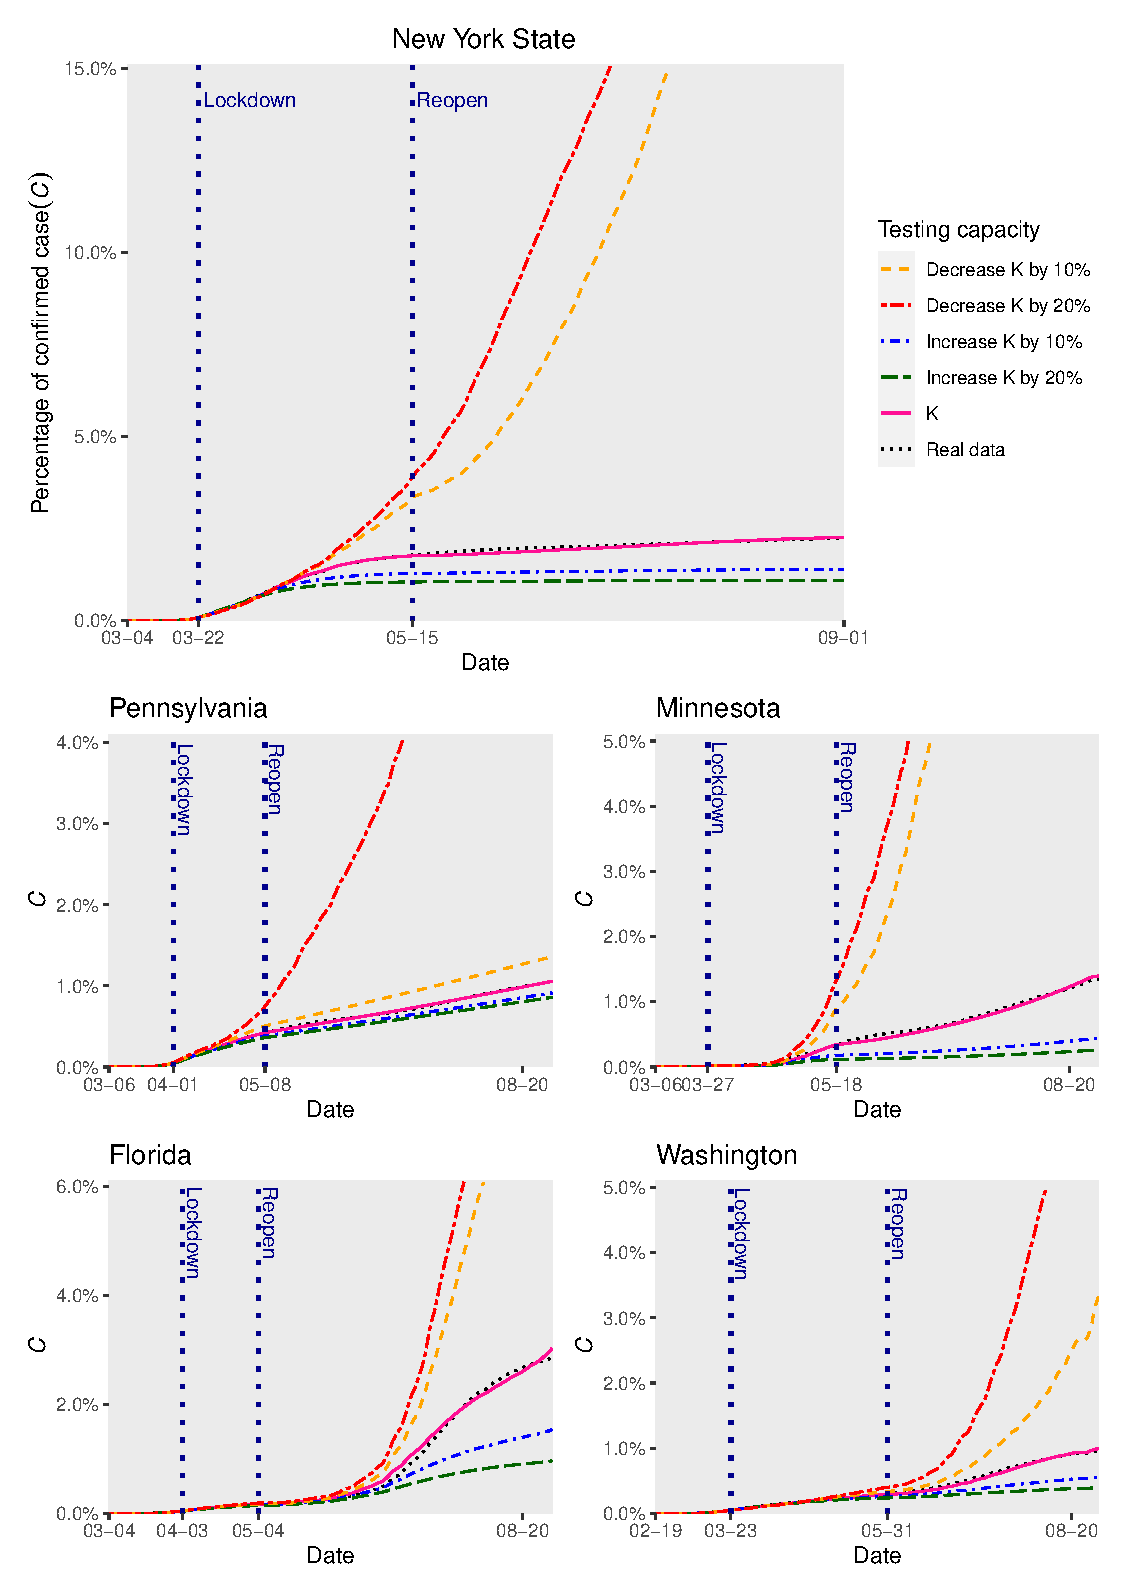
\includegraphics[width=0.8\linewidth, angle=0]{fivestates_1.eps}
\end{figure}

In Figure~\ref{fig:all states}, we show the predicted number of confirmed cases  using our model for different testing capacities.
The solid and dotted lines correspond to the model prediction and the actual data for $C_t$, respectively.
For all five states, the prediction matches the data reasonably well.
We also show the potential number of confirmed cases when the testing capacity had been increased/decreased by 10\%/20\% relative to the actual data.
%are the actual confirmed cases in each state reported in the data source, and the colored lines are our fitted results using different levels of testing capacity.
We explain the figure for New York as an example.
In New York, the first stage lasted from March 02, 2020, to March 22, 2020, and the second stage lasted from March 22, 2020, to May 15, 2020.
This is because the government announced that all non-essential business statewide must close in-office personnel functions effective at 8 pm on March 22, and started to reopen on May 15.
The marginal effect of adjusting the testing capacity is highly asymmetric.
While increasing $K$ by 20\% would approximately lower the total number of confirmed cases by 50\%, decreasing $K$ by 20\% would more than triple the total number of confirmed cases.
%Interestingly, when comparing the trajectories of decreasing $K$ by 10\% vs. 20\%, the number of confirmed cases, $C_t$, is fewer for a certain period (from the mid of June to the end) for the 20\% capacity decrease.
%This is because, in the short term, less testing may cause a smaller number of infected cases to be detected.
%For an extreme example, if the testing remains 100 cases per day, then the confirmed cases increase at most by 100 per day.
%It is a sign of severely insufficient testing instead of the slowdown of the disease.
As time proceeds, limited testing may lead to a large number of undetected infections and rapid spread of the disease.
This is indeed the case as we can show that the trajectory of the total infected cases (confirmed or not), $I_t+C_t$, of the 20\% reduction dominates that of the 10\% reduction.

Similarly, for the remaining four states, our model captures the patterns of confirmed cases in the data well.
This demonstrates the richness of our parsimonious model with only four parameters.
%\nc{Three or four?}
%we can see that after reopening, the number of confirmed cases in Pennsylvania and Minnesota has not grown too much. However, in Florida and Washington, the number of confirmed cases is still growing rapidly.


\begin{figure}[htbp]
	\centering
 	\caption{Changing $K$ and the resulting number of cases in New York on 2020/03/22}
 	\label{fig:ny k}
	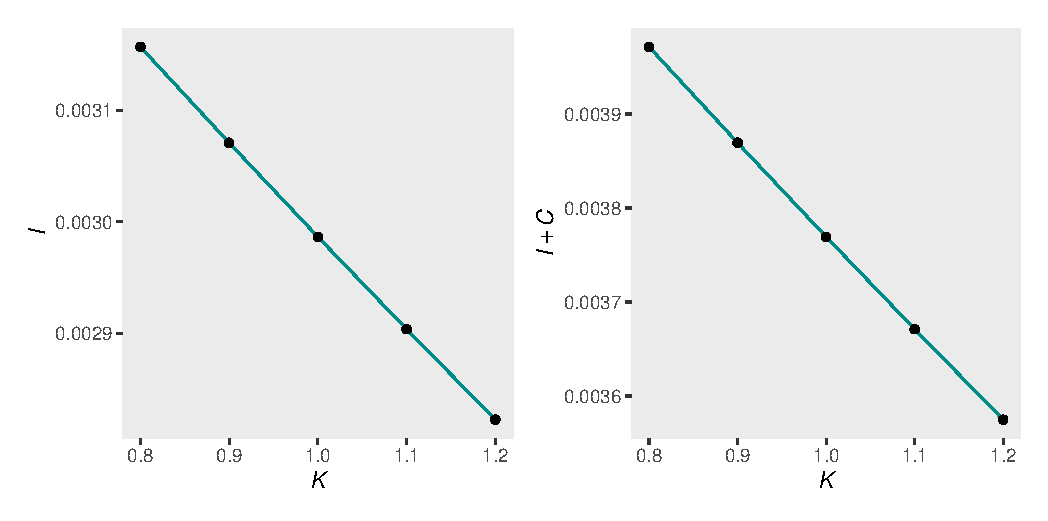
\includegraphics[width=0.75\linewidth, angle=0]{k.eps}
\end{figure}

\begin{figure}[htbp]
	\centering
 	\caption{Changing $\delta$ and the resulting number of cases in New York on 2020/03/22}
 	\label{fig:ny delta}
	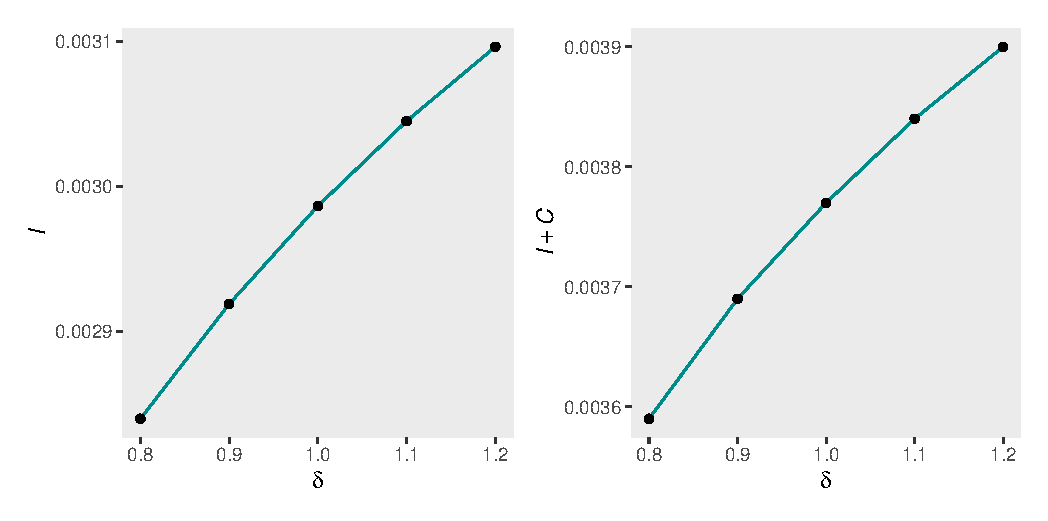
\includegraphics[width=0.75\linewidth, angle=0]{delta.eps}
\end{figure}

\begin{figure}[t]
	\centering
 	\caption{Changing $\gamma$ and the resulting number of cases in New York on 2020/03/22}
 	\label{fig:ny gamma}
	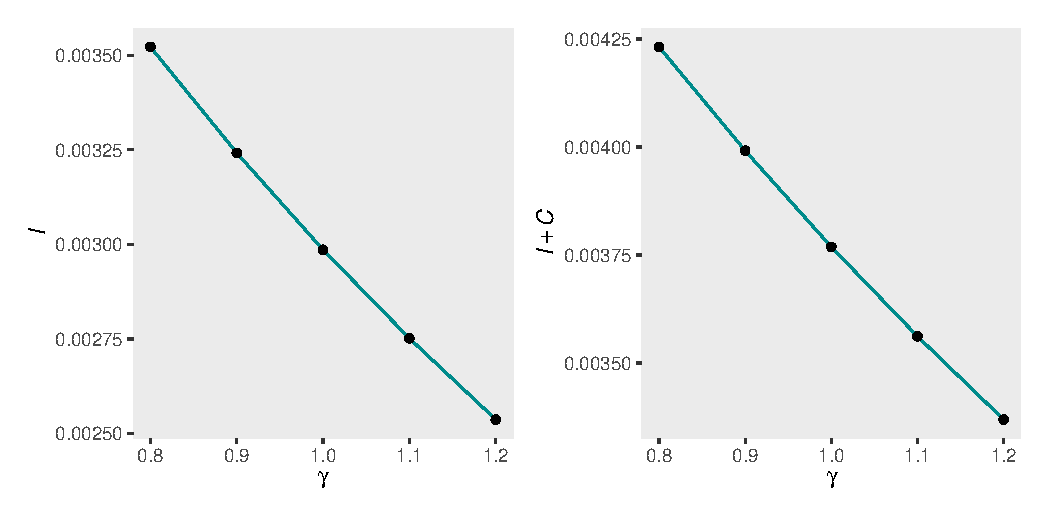
\includegraphics[width=0.75\linewidth, angle=0]{gamma.eps}
\end{figure}



\begin{figure}[ht]
	\centering
 	\caption{Changing $\beta$ and the resulting number of cases in New York on 2020/03/22}
 	\label{fig:ny beta}
	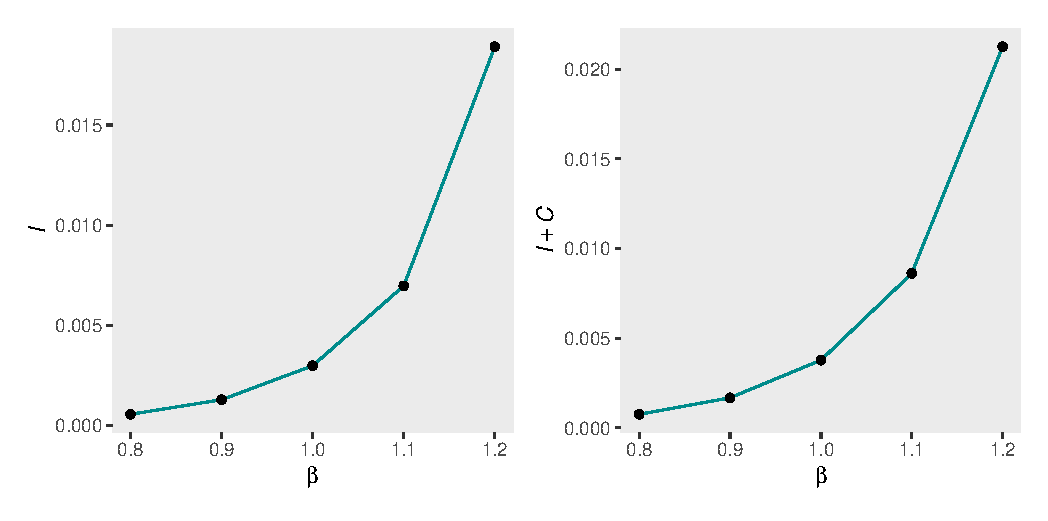
\includegraphics[width=0.75\linewidth, angle=0]{beta.eps}
\end{figure}

\begin{figure}[ht]
	\centering
 	\caption{Changing $\beta$ and $K$ simultaneously and the resulting number of cases in New York on 2020/03/22}
 	\label{fig:ny beta and k}
	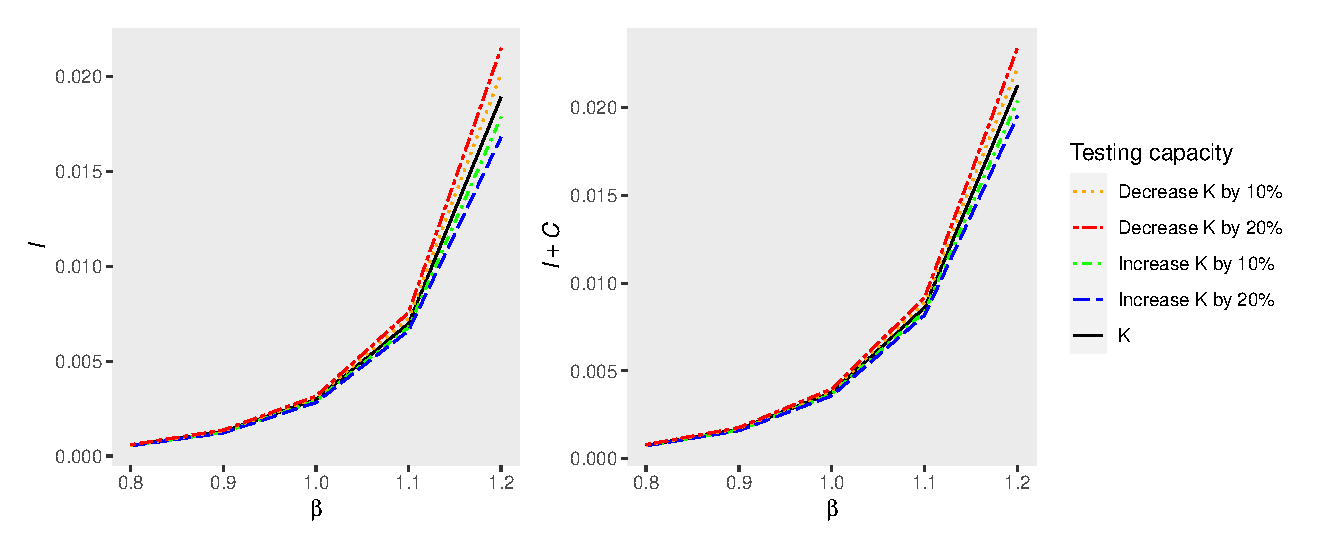
\includegraphics[width=0.9\linewidth, angle=0]{two_policies.eps}
\end{figure}

In addition, Figures~\ref{fig:ny k} to~\ref{fig:ny beta and k} show how the parameters influence the number of infections and confirmed cases.
Here we use the data from New York State on March 22, 2020, the last day of the first stage (Before Lockdown).
The goal is to numerically verify the structural properties in Propositions~\ref{prop:with k} to~\ref{prop:two policies}.
In particular, in Figure~\ref{fig:ny beta and k}, we numerically examine the cross-derivatives using finite differences in order to validate Proposition~\ref{prop:two policies}.
We find that the numerical results are consistent with the theoretical predictions, except for the right panel of Figure~\ref{fig:ny beta and k}, which contradicts the second part of Proposition~\ref{prop:two policies}.
This is probably due to the violation of the condition $\beta(1-s_0)\le\frac{1}{2}$.

%\cz{For Figure~\ref{fig:ny beta and k}, it is consistent with the first part of Proposition~\ref{prop:two policies} that $I_2$ has increasing differences in $K$ and $-\beta$. However, for the second part, when we increase $\beta$, the condition $\beta(1-s_0)\le\frac{1}{2}$ is no longer satisfied, thus $I_2+C_2$ does not have decreasing differences in $K$ and $-\beta$. }

\section{Concluding Remarks}
We build a parsimonious model to capture the impact of limited testing capacity on a disease diffusion process.
%It deviates from the usual approach in the literature that typically treats the limited testing as a testing rate that determines the transition from the infected but unconfirmed to the confirmed.
Our approach highlights the negative externality caused by testing the uninfected when the resources are already highly constrained, as the limited resources are shared among all who intend to get tested.
This simple model not only generates a set of subtle first- and second-order structural properties on system primitives which yield immediate policy implications, but also provides promising empirical predictions.
In fact, we demonstrate through the empirical study that modeling the testing capacity is crucial in understanding the development of COVID-19.
\cz{We also show the interactions between two commonly used policies: increasing testing capacity and quarantine/social distancing policies.}
With a few parameters, our model is able to fit the data as well as other compartmental models with a much higher degree of freedom.
This research leaves a lot to be desired in taking operational perspectives on the epidemic diffusion models and comparing the performance of models with and without more detailed operational views.


%\clearpage
\bibliographystyle{ormsv080}
\bibliography{covid19}

%%%%%%%%%%%%%%%%%%%%%%%%%%%%%%%%%%%%%%%%%%%%%%%%%%%%%%%%%%%%%%%%%%%%%%%%%%%%%%%%%%%%%%%%%%%%%%%%%%%%%%%%

\newpage
\setcounter{page}{1}

\counterwithin{equation}{section}
\counterwithin{table}{section}
\counterwithin{figure}{section}
\counterwithin{definition}{section}
\counterwithin{lemma}{section}
\counterwithin{proposition}{section}
\counterwithin{theorem}{section}
\counterwithin{corollary}{section}

\renewcommand\thesection{\Alph{section}}
\renewcommand\theequation{\Alph{section}.\arabic{equation}}
\renewcommand\thetable{\Alph{section}.\arabic{table}}
\renewcommand\thefigure{\Alph{section}.\arabic{figure}}
\renewcommand\thedefinition{\Alph{section}.\arabic{definition}}
\renewcommand\thelemma{\Alph{section}.\arabic{lemma}}
\renewcommand\theproposition{\Alph{section}.\arabic{proposition}}
\renewcommand\thetheorem{\Alph{section}.\arabic{theorem}}\renewcommand\thecorollary{\Alph{section}.\arabic{corollary}}

\setcounter{section}{0}
\setcounter{equation}{0}
\setcounter{table}{0}
\setcounter{figure}{0}
\setcounter{definition}{0}
\setcounter{lemma}{0}
\setcounter{proposition}{0}
\setcounter{theorem}{0}
\setcounter{corollary}{0}
\setcounter{footnote}{0}

%%%%%%%%%%%%%%%%%%%%%%%%%%%%%%%%%%%%%%%%%%%%%%%%%%%%%%%%%%%%%%%%%%%%%%%%%%%%%%%%%%%%%%%%%%%%%%%%%%%%%%%%

\begin{center}
	{\textbf{\large Online Appendix to\\
	``Capacitated SIR Model with an Application to COVID-19''}}
\end{center}
\section{Proofs of Results in Section~\ref{The Model}}
\label{Appendix Proofs of technical results}

\proof{Proof of Proposition \ref{prop:with k}.}

We first prove that $I_2$ is decreasing in $K$. Taking the first-order derivative of $I_2$ with respect to $K$, we have
%\begin{align}
%\frac{\partial I_2}{\partial K}&=\frac{\gamma\delta\eta  ADK}{(\gamma(1-D-\eta AK)+\delta D)^2}-\frac{\gamma(1-D-\eta AK)}{\gamma(1-D-\eta AK)+\delta D}-\eta A-\frac{A\beta D^2}{(1-\eta AK)^2}\notag\\
%&=-\eta A\left(1-\frac{\gamma\delta DK}{(\gamma(1-D-\eta AK)+\delta D)^2}\right)-\frac{\gamma(1-D-\eta AK)}{\gamma(1-D-\eta AK)+\delta D}-\frac{A\beta D^2}{(1-\eta AK)^2}\notag\\
%&=-\eta A\left(1-\gamma\frac{K}{\gamma(1-D-\eta AK)+\delta D}\frac{\delta D}{\gamma(1-D-\eta AK)+\delta D}\right)-\frac{\gamma(1-D-\eta AK)}{\gamma(1-D-\eta AK)+\delta D}\notag\\
%&\ \ \ -\frac{A\beta D^2}{(1-\eta AK)^2}.\label{eq:i2K}
%\end{align}

\begin{align}
\frac{\partial I_2}{\partial K}&=\frac{\gamma\delta  ADK}{(\gamma(1-D-AK)+\delta D)^2}-\frac{\gamma(1-D-AK)}{\gamma(1-D-AK)+\delta D}-A-\frac{A\beta D^2}{(1-AK)^2}\notag\\
&=-A\left(1-\frac{\gamma\delta DK}{(\gamma(1-D-AK)+\delta D)^2}\right)-\frac{\gamma(1-D-AK)}{\gamma(1-D-AK)+\delta D}-\frac{A\beta D^2}{(1-AK)^2}\notag\\
&=-A\left(1-\gamma\frac{K}{\gamma(1-D-AK)+\delta D}\frac{\delta D}{\gamma(1-D-AK)+\delta D}\right)-\frac{\gamma(1-D-AK)}{\gamma(1-D-AK)+\delta D}\notag\\
&\ \ \ -\frac{A\beta D^2}{(1-AK)^2}.\label{eq:i2K}
\end{align}

For the first term in \eqref{eq:i2K}, we show it is non-positive.
Because $K_t\le \delta S_t+\gamma I_t$, we have $\frac{K}{\delta S_1+\gamma I_1}\le1$.
Plugging in $S_1=D$ and $I_1=1-D-\eta AK$ yields
\begin{equation} \label{eq:fraction less than one}
\frac{K}{\gamma(1-D-\eta AK)+\delta D}\le 1.
\end{equation}
Moreover, because $I_1$ is non-negative, which is equivalent to
\begin{equation} \label{eq:I1positive}
1-D-AK\ge0,
\end{equation}
we have $\frac{\delta D}{\delta D+\gamma(1-D-\eta AK)}\le 1$.
Combining these inequalities together, it is easy to see that the first term in \eqref{eq:i2K} is non-positive.
%Since we assume $K_1=K_2=K$, then $\frac{K}{\gamma(1-D-AK)+\delta D}\le1$, and $\frac{\delta D}{\delta D+\gamma(1-D-AK)}\le1,\gamma\le1$, then $\gamma\frac{K}{\delta D+\gamma(1-D-AK)}\frac{\delta D}{\delta D+\gamma(1-D-AK)}\le1, A(1-\frac{\gamma K\delta D}{(\gamma(1-D-AK)+\delta D)^2})\ge0, -A(1-\frac{\gamma K\delta D}{(\gamma(1-D-AK)+\delta D)^2})\le0$.
For the second term in \eqref{eq:i2K}, it is non-positive because of \eqref{eq:I1positive}. Obviously, the third term in \eqref{eq:i2K} is non-positive, too.
Therefore, we have shown that \eqref{eq:i2K} is non-positive and thus $I_2$ is decreasing in $K$.



Next, we study the second-order derivative of $I_2$ with respect to $K$.
Note that
\begin{equation*}
\frac{\partial^2 I_2}{\partial K^2}=2AD\left(\frac{\gamma\delta(\gamma+(\delta-\gamma)D)}{(\gamma(1-D-AK)+\delta D)^3}-\frac{A\beta D}{(1-AK)^3}\right).
\end{equation*}
Denote $f(\delta)=\frac{\gamma\delta(\gamma+(\delta-\gamma)D)}{(\gamma(1-D-AK)+\delta D)^3}-\frac{A\beta D}{(1-AK)^3}.$ Since $2AD>0$, the sign of $\frac{\partial^2 I_2}{\partial K^2}$ and $f(\delta)$ are the same. Hence we only study the sign of $f(\delta)$. Recall that $A$ and $D$ are defined in \eqref{eq:AD-def}. Thus $A$ is a function of $\delta$ and $D$ is not.
When $\delta=0$, $f(0)=-\frac{A\beta D}{(1-AK)^3}<0$.
Since $f(\delta)$ is a continuous function of $\delta$, there exists $\epsilon_1>0$ such that $f(x)\le 0$ for $x\in(0,\epsilon_1)$.
When $\delta=\gamma$, $f(\gamma)=\frac{\gamma^3}{(\gamma(1-AK))^3}-\frac{A(1-\beta D)}{(1-K)^3}=\frac{1-A\beta D}{(1-AK)^3}$.
Because $A=\frac{\gamma(1-s_0)}{\gamma s_0+\gamma(1-s_0)}=1-s_0\le1$, $\beta\le1$, $D\le1$, we have $A\beta D\le1$, $1-A\beta D\ge0$.
Therefore, $f(\gamma)\ge0$.
By continuity, there exists $\epsilon_2>0$, such that $f(\gamma-x)\ge0$ for $x\in(0,\epsilon_2)$.


Then we prove that $I_2+C_2$ is decreasing in $K$. Recall that $I_2+C_2=1-S_2=1-D+\frac{\beta D(1-D-AK)}{1-AK}$. Taking the first-order derivative of $I_2+C_2$ with respect to $K$, we have
\begin{align*}
   \frac{\partial (I_2+C_2)}{\partial K}&=\beta D\frac{-A(1-AK)+A(1-D-AK)}{(1-AK)^2}\\
   &=-\frac{A\beta D^2}{(1-AK)^2}.
\end{align*}
Thus $\frac{\partial (I_2+C_2)}{\partial K}\le 0$,  i.e.,  $I_2+C_2$ is decreasing in $K$.

As for the concavity of $I_2+C_2$, taking the second-order derivative of $I_2+C_2$ with respect to $K$, we have
\begin{align*}
   \frac{\partial^2 (I_2+C_2)}{\partial K^2}=-\frac{2A^2\beta D^2}{(1-AK)^3}.
\end{align*}
Thus $\frac{\partial^2 (I_2+C_2)}{\partial K^2}\le 0$, i.e., $I_2+C_2$ is concave in $K$.\Halmos
\endproof





%%%%%%%%%%%%%%%%%%
\proof{Proof of Proposition \ref{prop:with delta}.}
We first prove that $I_2$ is increasing in $\delta$.
Recall that
\begin{align*}
I_2&=-\frac{\gamma K(1-D-AK)}{\delta D+\gamma(1-D-AK)}+1-D-AK+\frac{\beta D(1-D-AK)}{1-AK}\\
&=1-(A+1)K-(1-\beta)D-\frac{\beta D^2}{1-AK}+\frac{\delta DK}{\gamma(1-D-AK)+\delta D}.
\end{align*}
By \eqref{eq:AD-def}, $A$ is a function of $\delta$ while $D$ is not. Taking the first-order derivative of $A$ with respect to $\delta$, we have
\begin{equation}\label{eq:Adelta-deriv}
   \frac{\partial A}{\partial\delta}=\frac{-\gamma s_0(1-s_0)}{(\gamma(1-s_0)+\delta s_0)^2}=\frac{-A(1-A)}{\delta}.
\end{equation}
Therefore,
\begin{align}
\frac{\partial I_2}{\partial \delta}&=\frac{KA(1-A)}{\delta}+\frac{\beta D^2KA(1-A)}{\delta(1-AK)^2}-\frac{\gamma DK^2A(1-A)}{(\gamma(1-D-AK)+\delta D)^2}+\frac{\gamma DK(1-D-AK)}{(\gamma(1-D-AK)+\delta D)^2}\notag\\
&=\frac{KA(1-A)}{\delta}\left(1-\frac{\gamma\delta DK}{(\gamma(1-D-AK)+\delta D)^2}\right)+\frac{\beta D^2 KA(1-A)}{\delta(1-AK)^2}+\frac{\gamma DK(1-D-AK)}{(\gamma(1-D-AK)+\delta D)^2}.\label{eq:I2delta}
\end{align}
To show the first term is non-negative in \eqref{eq:I2delta}, it is sufficient to show
\begin{equation}
\label{eq:postive}
1-\frac{\gamma\delta DK}{(\gamma(1-D-AK)+\delta D)^2}=1-\gamma\frac{\delta D}{\gamma(1-D-AK)+\delta D}\frac{K}{\gamma(1-D-AK)+\delta D}
\end{equation}
is non-negative.
By \eqref{eq:I1positive}, we have $\gamma(1-D-AK)+\delta D\ge \delta D$ and $\frac{\delta D}{\gamma(1-D-AK)+\delta D}\le 1$.
By \eqref{eq:fraction less than one}, we have $\frac{K}{\gamma(1-D-AK)+\delta D}\le 1$. Combined with $\gamma\le 1$, we can show the first term is non-negative.
The second and third terms in \eqref{eq:I2delta} are both non-negative by the definition of the parameters.
Therefore, we have $\frac{\partial I_2}{\partial \delta}\ge0$. Thus $I_2$ is increasing in $\delta$.

Next, we are going to show the concavity of $I_2$. Taking the second-order derivative of $I_2$ with respect to $\delta$, we have
\begin{align}
    \frac{\partial^2 I_2}{\partial \delta^2}=&-\frac{2KA(1-A)^2}{\delta^2}-\frac{2\beta D^2KA(1-A)^2}{\delta^2(1-AK)^2}-\frac{(1-A)(A+2K)}{\delta(\gamma(1-D-AK)+\delta D)^2}\notag\\
    &-\frac{2(\gamma KA(1-A)+\delta D)(1-D- KA(2-A))}{\delta(\gamma(1-D-AK)+\delta D)^3}.\label{eq:I2delta second derivative}
\end{align}
The first, second and third terms in \eqref{eq:I2delta second derivative} are non-positive by the definition of parameters.
For the fourth term in \eqref{eq:I2delta second derivative}, it is sufficient to show that $1-D-KA(2-A)\ge0$. By \eqref{eq:AD-def}, $A\le1$, and thus $A(2-A)\le 1$. Hence, we have $1-D-KA(2-A)\ge1-D-K$.
Since \eqref{eq:I1positive} holds for every $A$, we set $s_0=1$, and thus $A=1$. This implies that $1-D-K\ge0$. Hence, $1-D-KA(2-A)\ge1-D-K\ge0$.
Therefore, the fourth term in \eqref{eq:I2delta second derivative} is also non-negative and we have completed the proof of that $I_2$ is increasing and concave in $\delta$.

Next, we prove that $I_2+C_2$ is increasing in $\delta$.
Recall that $I_2+C_2=1-S_2=1-D+\frac{\beta D(1-D-AK)}{1-AK}$. By \eqref{eq:Adelta-deriv}, we have $\frac{\partial A}{\partial\delta}=\frac{-A(1-A)}{\delta}$. Taking the first-order derivative of $I_2+C_2$ with respect to $\delta$, we have
\begin{align}\label{eq:i2c2-delta}
    \frac{\partial (I_2+C_2)}{\partial \delta}&=\beta D\frac{-K\frac{\partial A}{\partial\delta}(1-AK)+K\frac{\partial A}{\partial\delta}(1-D-AK)}{(1-AK)^2}\notag\\
    &=-\frac{\beta D^2K\frac{\partial A}{\partial\delta}}{(1-AK)^2}\notag\\
    &=\frac{\beta D^2KA(1-A)}{\delta(1-AK)^2}.
\end{align}
By \eqref{eq:AD-def}, we have $1-A\ge0$, and hence, \eqref{eq:i2c2-delta} is non-negative. It implies that $I_2+C_2$ is increasing in $\delta$.

Then we are going to prove that $I_2+C_2$ is concave in $\delta$. Taking the second-order derivative of $I_2+C_2$ with respect to $\delta$, we have
\begin{align}\label{eq:i2c2-second deriv}
    \frac{\partial^2 (I_2+C_2)}{\partial \delta^2}&=-\beta D^2K\frac{(1-AK)^2\frac{\partial^2 A}{\partial \delta^2}+2K(1-AK)(\frac{\partial A}{\partial \delta})^2}{(1-AK)^4}\notag\\
    &=-\beta D^2K\frac{(1-AK)\frac{2A(1-A)^2}{\delta^2}+2K(\frac{A(1-A)}{\delta})^2}{(1-AK)^3}\notag\\
    &=-\frac{2\beta D^2KA(1-A)^2}{\delta^2(1-AK)^3}.
\end{align}
Now it is obvious that $\frac{\partial^2 (I_2+C_2)}{\partial \delta^2}\le0$, i.e., $I_2+C_2$ is concave in $\delta$.\Halmos
\endproof

\proof{Proof of Proposition \ref{prop:with gamma}.}
First, we prove $I_2$ is decreasing in $\gamma$. Taking the first-order derivative of $I_2$ with respect to $\gamma$, we have
\begin{equation}\label{eq:I2gamma}
\frac{\partial I_2}{\partial \gamma}
=-\frac{\delta KD(1-D-AK)}{(\delta D+\gamma(1-D-AK))^2}-\left(1-\frac{\delta\gamma KD}{(\delta D+\gamma(1-D-AK))^2}+\frac{\beta D^2}{(1-AK)^2}\right)\frac{\delta Ks_0(1-s_0)}{(\delta s_0+\gamma(1-s_0))^2}.
\end{equation}
The first term in \eqref{eq:I2gamma} is non-positive because of \eqref{eq:I1positive}.
For the second term in \eqref{eq:I2gamma}, recall that we have already proved $1-\frac{\delta\gamma KD}{[\gamma(1-D-AK)+\delta D]^2}\ge 0$
in \eqref{eq:postive}. Therefore $1-\frac{\delta\gamma KD}{[\gamma(1-D-AK)+\delta D]^2}+\frac{\beta D^2}{(1-AK)^2}\ge 0$ and the second term in \eqref{eq:I2gamma} is non-positive.
As a result, $\frac{\partial I_2}{\partial \gamma}\le 0$ and $I_2$ is decreasing in $\gamma$.

Next, we investigate the second-order property. Taking the second-order derivative of $I_2$ with respect to $\gamma$, we have
\begin{align}
 \frac{\partial^2 I_2}{\partial \gamma^2}
=&2\delta K s_0(1-s_0)^2\left(\frac{1}{(\gamma(1-s_0)+\delta s_0)^3}+\frac{\beta D^2(1-K)}{(\gamma(1-s_0)(1-K)+\delta s_0)^3}\right)\notag\\
&+\frac{2\delta^2 DK^2s_0(1-s_0)}{(\gamma(1-D-AK)+\delta D)^2(\gamma(1-s_0)+\delta s_0)^2}\left(1-\frac{\gamma(1-s_0)}{\gamma(1-s_0)+\delta s_0}\right)\notag\\
&+\frac{2\delta DK\left(1-D-AK-\frac{\delta\gamma Ks_0(1-s_0)}{(\gamma-\gamma s_0+\delta s_0)^2}\right)^2}{(\gamma(1-D-AK)+\delta D)^3}.\label{eq:I2gamma second derivative}
\end{align}
It is easy to see that all the terms in \eqref{eq:I2gamma second derivative} are non-negative as we arrange them in the above way.
Therefore, $I_2$ is convex in $\gamma$.
%For the first term in \eqref{eq:I2gamma second derivative}, since $1-s_0\ge 0, 1-K\le 0$, we have $\frac{1}{[\gamma(1-s_0)+\delta s_0]^3}+\frac{\beta D^2(1-K)}{[\gamma(1-s_0)(1-K)+\delta s_0]^3}\ge 0$, so the first term is non-negative. For the second and third term in \eqref{eq:I2gamma second derivative}, they are obviously also non-negative. Thus $\frac{\partial^2 I_2}{\partial \gamma^2}\ge 0$. $I_2$ is a convex function about $\gamma$.

Now, we prove $I_2+C_2$ is decreasing in $\gamma$. Recall that $I_2+C_2=1-S_2=1-D+\frac{\beta D(1-D-AK)}{1-AK}$. By \eqref{eq:Adelta-deriv}, we have $\frac{\partial A}{\partial\gamma}=\frac{A(1-A)}{\gamma}$ and thus
%\nc{The next label is multiply defined.}
\begin{align*}%\label{eq:i2c2-gamma}
    \frac{\partial (I_2+C_2)}{\partial \gamma}&=\beta D\frac{-K\frac{\partial A}{\partial\gamma}(1-AK)+K\frac{\partial A}{\partial\gamma}(1-D-AK)}{(1-AK)^2}=-\frac{\beta D^2K\frac{\partial A}{\partial\gamma}}{(1-AK)^2}=-\frac{\beta D^2KA(1-A)}{\gamma(1-AK)^2}.
\end{align*}
It is easy to see that $\frac{\partial (I_2+C_2)}{\partial \gamma}\le 0$, thus $I_2+C_2$ is decreasing in $\gamma$.
Finally, we prove the convexity of $I_2+C_2$.
\begin{align*}
    \frac{\partial^2 (I_2+C_2)}{\partial \gamma^2}&=-\beta D^2K\frac{(1-2A)\frac{\partial A}{\partial\gamma}\gamma(1-AK)^2-A(1-A)(1-AK)(1-3AK+2A^2K)}{\gamma^2(1-AK)^4}\notag\\
    &=-\beta D^2K\frac{(1-2A)A(1-A)(1-AK)^2-A(1-A)(1-AK)(1-3AK+2A^2K)}{\gamma^2(1-AK)^4}\notag\\
    &=-\beta D^2K\frac{A(1-A)(1-AK)((1-2A)(1-AK)-1+3AK-2A^2K)}{\gamma^2(1-AK)^4}\\
    &=\frac{2\beta D^2KA^2(1-A)(1-AK)(1-K)}{\gamma^2(1-AK)^4}.
\end{align*}
Now it is obvious that $\frac{\partial^2 (I_2+C_2)}{\partial \gamma^2}$ is non-negative. Thus $I_2+C_2$ is convex in $\gamma$.\Halmos
\endproof


\proof{Proof of Proposition \ref{prop:with beta}.}
First we prove that $I_2+C_2$ is increasing in $\beta$. Recall that $I_2+C_2=1-S_2=1-D+\frac{\beta D(1-D-AK)}{1-AK}$, where $D=\beta s_0^2+(1-\beta)s_0=s_0-\beta s_0(1-s_0)$. By \eqref{eq:Adelta-deriv}, we have $\frac{\partial D}{\partial\beta}=-s_0(1-s_0)$. Taking the first-order derivative of $I_2+C_2$ with respect to $\beta$, we have
\begin{align*}
    \frac{\partial (I_2+C_2)}{\partial \beta}&=s_0(1-s_0)+\frac{D(1-D-AK)+\beta(1-2D-AK)\frac{\partial D}{\partial\beta}}{1-AK}\notag\\
    &=s_0(1-s_0)+\frac{D(1-D-AK)-\beta s_0(1-s_0)(1-2D-AK)}{1-AK}\notag\\
    &=s_0(1-s_0)+\frac{D(1-D-AK)+\beta s_0(1-s_0)(D-(1-D-AK))}{1-AK}.
\end{align*}
At the beginning of the epidemic, the number of infected people will not exceed the number of healthy people. Thus it is reasonable to assume that at $t=1$,
\begin{equation}\label{eq:s1i1-relation}
    S_1-I_1\ge0,
\end{equation}
which is $D-(1-D-AK)\ge0$. With this assumption, it is not difficult to see that $\frac{\partial (I_2+C_2)}{\partial \beta}\ge0$. Thus $I_2+C_2$ is increasing in $\beta$.

Then we investigate the second-order property of $I_2+C_2$ with respect to $\beta$.
\begin{align*}
    \frac{\partial^2 (I_2+C_2)}{\partial \beta^2}&=(\frac{\partial D}{\partial\beta}+\frac{s_0(1-s_0)}{1-AK}(-1+2D+AK+2\beta\frac{\partial D}{\partial\beta})\\
    &=\frac{2s_0(1-s_0)}{1-AK}(\beta s_0(1-s_0)+D-(1-AK-D))\\
    &=\frac{2s_0(1-s_0)}{1-AK}(S_1-S_0+S_1-I_1).
\end{align*}
Since we have $S_0\ge S_1\ge I_1$, if $2S_1\ge S_0+I_1$, then $I_2+C_2$ is convex in $\beta$. Otherwise, $I_2+C_2$ is concave in $\beta$.\Halmos

\proof{Proof of Proposition \ref{prop:two policies}}
First we prove that $\frac{\partial I_2}{\partial K\partial\beta}\le0$. Recall that $I_2=1-(A+1)K-(1-\beta)D-\frac{\beta D^2}{1-AK}+\frac{\delta DK}{\gamma(1-D-AK)+\delta D}$. Taking the derivative of $I_2$ with respect to $K$ and $\beta$, we have
\begin{align}\label{eq:i2-k and beta}
    \frac{\partial^2 I_2}{\partial K\partial\beta}&=-\delta\gamma s_0(1-s_0)\frac{(1-2\eta AK)(\delta D+\gamma(1-D-\eta AK))+2\eta\gamma AK}{(\delta D+\gamma(1-D-\eta AK))^3}-\eta A\frac{D^2-2\beta Ds_0(1-s_0)}{(1-\eta AK)^2}\notag\\
    &=-\delta\gamma s_0(1-s_0)\frac{\delta D+\gamma(1-D-\eta AK)+2\eta ADK(\gamma-\delta)}{(\delta D+\gamma(1-D-\eta AK))^3}-\eta AD\frac{2s_0-D}{(1-\eta AK)^2}.
\end{align}
The first term in \eqref{eq:i2-k and beta} is non-positive because of \eqref{eq:I1positive} and the previous condition $\gamma\ge\delta$. For the second term in \eqref{eq:i2-k and beta}, by \eqref{eq:AD-def}, $2s_0-D=2s_0-(s_0-\beta s_0(1-s_0))=s_0+\beta s_0(1-s_0)\ge0$. Hence, the second term in \eqref{eq:i2-k and beta} is also non-positive. Therefore, $\frac{\partial I_2}{\partial K\partial\beta}\le0$.

Next, we prove that $\frac{\partial (I_2+C_2)}{\partial K\partial\beta}\ge0$. Recall that $I_2+C_2=1-S_2=1-D+\frac{\beta D(1-D-AK)}{1-AK}$, where $D=\beta s_0^2+(1-\beta)s_0=s_0-\beta s_0(1-s_0)$.
Taking the derivative of $I_2+C_2$ with respect to $K$ and $\beta$, we have
\begin{align*}%\label{eq:i2c2-k and beta}
    \frac{\partial^2 (I_2+C_2)}{\partial K\partial\beta}&=\frac{\eta A}{(1-\eta AK)^2}(D(1-D)-\beta s_0(1-s_0)(1-2D))\notag\\
    &=\frac{\eta A}{(1-\eta AK)^2}((1-D)(2D-s_0)+D(s_0-D))\notag\\
    &=\frac{\eta A}{(1-\eta AK)^2}((1-D)(s_0-2\beta s_0(1-s_0))+D(s_0-D)).
\end{align*}
If $\beta(1-s_0)\le\frac{1}{2}$, then $(1-D)(s_0-2\beta s_0(1-s_0))\ge0$. By \eqref{eq:AD-def}, $D\le s_0$, thus $D(s_0-D)\ge0$. Hence, we have $\frac{\partial I_2+C_2}{\partial K\partial\beta}\ge0$.\Halmos



\endproof

\section{Structural Properties for $t>2$}
\label{Appendix Proofs of extensions of four propositions}
In this section, we explore the structural properties of our model when $t>2$, complementing the results in Section~\ref{The Model}.
Because of the complexity of the model, we present our result in the form of mathematical induction.
In particular, the structural results in Section~\ref{The Model} provide the base case for the induction.
Next, we provide a set of conditions for the inductive step to possibly carry forward.

\begin{proposition}
\label{Extensions with K}
For $t\ge2$, suppose $I_{t}$ and $I_{t}+C_{t}$ are decreasing and concave in $K$, if $|I_{t}'|\ge|S_{t}'|$, $|I_{t}''|\ge|S_{t}''|$, $S_{t}\ge I_{t}$, and $K\le-\frac{I_{t}}{I_{t}'}$,
%If $K\le-\frac{I_{t}}{I_{t}'}$ and $K\ge\frac{\delta(S_{t}'I_{t}-2S_{t}I_{t}')-\gamma I_{t}I_{t}'}{I_{t}''(\delta S_{t}+\gamma I_{t})-I_{t}'(\delta S_{t}'+\gamma I_{t}')}$,
then $I_{t+1}$ and $I_{t+1}+C_{t+1}$ are decreasing and concave in $K$.
\end{proposition}

\proof{Proof of Proposition \ref{Extensions with K}.}

First we prove that $I_{t+1}$ and $I_{t+1}+C_{t+1}$ are decreasing in $K$.
When $I_t$ is decreasing in $K$ and $S_t$ is increasing in $K$ for $t\ge2$, then $I_t'\le 0$, $S_t'\ge 0$. We also have $S_t\ge I_t$ and $|I_t'|\ge|S_t'|$. Then, for $S_{t+1}(K)$, we have
\begin{equation}\label{eq:st+1}
    S_{t+1}(K)=S_{t}(K)-\frac{\beta I_{t}(K)S_{t}(K)}{S_{t}(K)+I_{t}(K)}.
\end{equation}
For $I_{t+1}(K)$, we have
\begin{equation}\label{eq:it+1}
    I_{t+1}(K)=\frac{\beta I_{t}(K)S_{t}(K)}{S_{t}(K)+I_{t}(K)}+I_{t}(K)-\eta K\frac{\gamma I_{t}(K)}{\delta S_{t}(K)+\gamma I_{t}(K)}.
\end{equation}
Taking the first-order derivative of $S_{t+1}$ with respect to $K$, we have
\begin{equation*}
    \frac{\partial S_{t+1}}{\partial K}=S_{t}'-\beta\frac{S_{t}^2I_t'+I_{t}^2S_t'}{(S_{t}+I_{t})^2}.
\end{equation*}
Taking the first-order derivative of $I_{t+1}$ with respect to $K$, we have
\begin{align}
    \frac{\partial I_{t+1}}{\partial K}&=\beta\frac{S_{t}^2I_t'+I_{t}^2S_t'}{(S_{t}+I_{t})^2}+I_t'-\eta\frac{\gamma I_t+\gamma KI_t'}{\delta S_{t}+\gamma I_{t}}+\frac{\eta\gamma KI_t(\delta S_{t}'+\gamma I_{t}')}{(\delta S_{t}+\gamma I_{t})^2}\notag\\
    &=\beta\frac{S_{t}^2I_t'+I_{t}^2S_t'}{(S_{t}+I_{t})^2}+I_t'(1-\frac{\eta\gamma K}{\delta S_{t}+\gamma I_{t}})-\eta\frac{\gamma I_t}{\delta S_{t}+\gamma I_{t}}+\frac{\eta\gamma KI_t(\delta S_{t}'+\gamma I_{t}')}{(\delta S_{t}+\gamma I_{t})^2}.\label{eq:it with k}
\end{align}

We next show $S_{t+1}'(K)\ge0$.
For the first term in $\frac{\partial S_{t+1}}{\partial K}$, we already assume that $S_t'\ge0$, and hence, the first term is non-negative. We also assume that most people are healthy, which is $S_{t}\ge I_{t}$.
Thus for the second term in $\frac{\partial S_{t+1}}{\partial K}$, we have $S_{t}^2>I_{t}^2$. We also have $I_t'\le 0$, $S_t'\ge 0$ and $|I_{t}'|\ge|S_{t}'|$. Thus
\begin{equation}\label{eq:st it with derivative}
    S_{t}^2I_t'(K)+I_{t}^2S_t'(K)\le0.
\end{equation}
The second term is non-negative. Thus we have $S_{t+1}'\ge0$. Because $S_{t+1}+I_{t+1}+C_{t+1}=1$, $I_{t+1}'+C_{t+1}'=-S_{t+1}'\le0$. Thus $I_{t+1}+C_{t+1}$ is decreasing in $K$.

We next show $I_{t+1}'\ge0$.
For the first term in \eqref{eq:it with k}, by \eqref{eq:st it with derivative}, the first term is non-positive. For the second term in \eqref{eq:it with k}, since we have assumed testing supply is below demand, which is $\frac{K}{\delta S_{t}+\gamma I_{t}}\le1$, we have
\begin{equation}\label{eq:testing capacity general}
    1-\frac{\eta\gamma K}{\delta S_{t}+\gamma I_{t}}\ge0.
\end{equation}
We also know that $I_t'\le0$. Thus the second term is also non-positive. The third term in \eqref{eq:it with k} is obviously non-positive. For the fourth term in \eqref{eq:it with k}, we assume that $\gamma\ge\delta$, which means the proportion of infected people get tested is greater than that of susceptible population. Then combining this condition with $I_t'(K)\le 0$, $S_t'(K)\ge 0$ and $|I_{t}'(K)|\ge|S_{t}'(K)|$, we have $\delta S_{t}'(K)+\gamma I_{t}'(K)\le0$. Thus the fourth term in \eqref{eq:it with k} is non-positive. Hence, we have $I_{t+1}'(K)\le0$, i.e., $I_{t+1}$ is decreasing in $K$.
%If the testing capacity satisfies that $K\le-\frac{I_t}{I_t'}$, then we have $-\eta\frac{\gamma I_t+\gamma KI_t'}{\delta S_{t}}\le0$. Thus $|I_{t+1}'(K)|\ge-\beta\frac{S_{t}^2I_t'+I_{t}^2S_t'}{(S_{t}+I_{t})^2}-I_t'\ge-\beta\frac{S_{t}^2I_t'+I_{t}^2S_t'}{(S_{t}+I_{t})^2}+S_t'=|S_{t+1}'(K)|$.
%Thus we have proved that $I_{t}'(K)\le0$ and $S_{t}'(K)\ge0$ holds for every $t\in\mathbb{N}$ if $K\le-\frac{I_{t-1}}{I_{t-1}'}$. Since $S_{t}'(K)+I_{t}'(K)+C_{t}'(K)=0$, so when $S_{t}'(K)\ge0$, $I_{t}'(K)+C_{t}'(K)\le0$.

Next, we investigate the second-order property of $I_t$ and $I_{t}+C_{t}$.
Taking the second-order derivative of $S_{t+1}$ with respect to $K$, we have
\begin{align}
    \frac{\partial^2 S_{t+1}}{\partial K^2}&=S_{t}''-\beta\frac{(2S_{t}S_{t}'I_{t}'+S_{t}^2I_{t}''+2I_{t}S_{t}'I_{t}'+I_{t}^2S_{t}'')(S_{t}+I_{t})-2(S_{t}^2I_{t}'+I_{t}^2S_{t}')(S_{t}'+I_{t}')}{(S_{t}+I_{t})^3}\notag\\
    &=S_{t}''-\beta\frac{-2(I_{t}S_{t}'-S_{t}I_{t}')^2+(S_{t}^2I_{t}''+I_{t}^2S_{t}'')(S_{t}+I_{t})}{(S_{t}+I_{t})^3}.\label{eq:s2k}
\end{align}
The first term in \eqref{eq:s2k} is non-negative because $S_t''\ge0$. For the second term in \eqref{eq:s2k}, since $S_t\ge I_t$ and $|I_{t}''|\ge|S_{t}''|$, we have $S_{t}^2I_{t}''+I_{t}^2S_{t}''\le0$, and the second term is non-negative. Thus we have $\frac{\partial^2 S_{t+1}}{\partial K^2}\ge0$. Because $S_{t+1}+I_{t+1}+C_{t+1}=1$, $I_{t+1}''+C_{t+1}''=1-S_{t+1}''\le0$. Thus $I_{t+1}+C_{t+1}$ is concave in $K$.

Next, we take the second-order derivative of $I_{t+1}$ with respect to $K$:
\begin{align}
    \frac{\partial^2 I_{t+1}}{\partial K^2}&=\beta\frac{-2(I_{t}S_{t}'-S_{t}I_{t}')^2+(S_{t}^2I_{t}''+I_{t}^2S_{t}'')(S_{t}+I_{t})}{(S_{t}+I_{t})^3}-\eta\gamma\frac{(2I_{t}'+KI_{t}'')(\delta S_{t}+\gamma I_{t})-(I_{t}+KI_{t}')(\delta S_{t}'+\gamma I_{t}')}{(\delta S_{t}+\gamma I_{t})^2}\notag\\
    &\ \ +I_{t}''+\eta\gamma\frac{\left((I_{t}+KI_{t}')(\delta S_{t}'+\gamma I_{t}')+KI_{t}(\delta S_{t}''+\gamma I_{t}'')\right)(\delta S_{t}+\gamma I_{t})-2KI_{t}(\delta S_{t}'+\gamma I_{t}')^2}{(\delta S_{t}+\gamma I_{t})^3}\notag\\
    &=\beta\frac{-2(I_{t}S_{t}'-S_{t}I_{t}')^2+(S_{t}^2I_{t}''+I_{t}^2S_{t}'')(S_{t}+I_{t})}{(S_{t}+I_{t})^3}+I_{t}''(1-\frac{\eta\gamma K}{\delta S_{t}+\gamma I_{t}})+\eta\gamma\frac{KI_{t}(\delta S_{t}''+\gamma I_{t}'')}{(\delta S_{t}+\gamma I_{t})^2}\notag\\
    &\ \ -2\eta\gamma\frac{KI_{t}(\delta S_{t}'+\gamma I_{t}')^2+I_{t}'(\delta S_{t}+\gamma I_{t})^2-(I_{t}+KI_{t}')(\delta S_{t}'+\gamma I_{t}')(\delta S_{t}+\gamma I_{t})}{(\delta S_{t}+\gamma I_{t})^3}.\label{eq:itk second derivative}
\end{align}
For the first term in \eqref{eq:itk second derivative}, by \eqref{eq:s2k}, this term is non-positive.
For the second term in \eqref{eq:itk second derivative}, we know $I_t''\le0$, and we have proved $(1-\frac{\eta\gamma K}{\delta S_{t}+\gamma I_{t}})\ge0$, so the second term is also non-positive. For the third term in \eqref{eq:itk second derivative}, since we have assumed $\gamma\ge\delta$, and $|I_{t}''|\ge|S_{t}''|$, so $|\gamma I_{t}''|\ge|\delta S_{t}''|$, $\gamma I_{t}''\le0$, $\delta S_{t}''\ge0$. Then we have $\delta S_{t}''+\gamma I_{t}''\le0$, the third term is also non-positive. Thus for the fourth term in \eqref{eq:itk second derivative}, $KI_{t}(\delta S_{t}'+\gamma I_{t}')^2+I_{t}'(\delta S_{t}+\gamma I_{t})^2\ge0$. Since $K\le-\frac{I_{t}}{I_{t}'}$, then $I_{t}+KI_{t}'\ge0$.
We have already proved that $\delta S_{t}'+\gamma I_{t}'\le0$, so the fourth term in \eqref{eq:itk second derivative} is also non-positive. Hence $\frac{\partial^2 I_{t+1}}{\partial K^2}\le0$, i.e., $I_{t+1}$ is concave in $K$.\Halmos
\endproof

\begin{proposition}
\label{Extensions with delta}
For $t\ge2$, suppose $I_{t}$ and $I_{t}+C_{t}$ are increasing and concave in $\delta$, $S_{t}\ge I_{t}$, $|S_{t}'|\le |I_{t}'|$, $|S_{t}''|\le |I_{t}''|$,
and $\delta\le\min\left\{\frac{S_{t}I_{t}}{S_{t}I_{t}'-S_{t}'I_{t}},\frac{2S_{t}'I_{t}}{S_{t}I_{t}''-S_{t}''I_{t}}\right\}$.
Then $I_{t+1}$ and $I_{t+1}+C_{t+1}$ are increasing and concave in $\delta$.
%When $\delta\le\frac{2S_{t-1}'I_{t-1}}{S_{t-1}I_{t-1}''-S_{t-1}''I_{t-1}}$, both $I_t$ and $I_t+C_t$ are concave in $\delta$.
\end{proposition}

\proof{Proof of Proposition \ref{Extensions with delta}.}

%For the induction step, suppose $I_t$ is increasing in $\delta$ and $S_t$ is decreasing in $\delta$ for some positive integer $t\ge2$, which is $I_t'(\delta)\ge 0$, $S_t'(\delta)\le 0$. We also suppose that $|\frac{\partial I_t}{\partial \delta}|\ge|\frac{\partial S_t}{\partial \delta}|$.
%By \eqref{eq:st+1} and \eqref{eq:it+1}, taking the first-order derivative of $S_{t+1}$ with respect to $\delta$, we have
First we prove that $I_{t+1}$ and $I_{t+1}+C_{t+1}$ are increasing in $\delta$.
When $I_t$ is increasing in $\delta$ and $S_t$ is decreasing in $\delta$ for $t\ge2$, $I_t'\ge 0$, $S_t'\le 0$. We also have $S_t\ge I_t$ and $|I_t'|\ge|S_t'|$. Then, for $S_{t+1}$, we have
\begin{equation}\label{eq:st with delta}
    \frac{\partial S_{t+1}}{\partial \delta}=S_{t}'-\beta\frac{S_{t}^2I_t'+I_{t}^2S_t'}{(S_{t}+I_{t})^2}.
\end{equation}
Taking the first-order derivative of $I_{t+1}$ with respect to $\delta$, we have
\begin{align}
    \frac{\partial I_{t+1}}{\partial \delta}&=\beta\frac{S_{t}^2I_t'+I_{t}^2S_t'}{(S_{t}+I_{t})^2}+I_t'-\eta\frac{\gamma KI_t'(\delta S_{t}+\gamma I_{t})-\gamma KI_t(S_{t}+\delta S_{t}'+\gamma I_{t}')}{(\delta S_{t}+\gamma I_{t})^2}\notag\\
    &=\beta\frac{S_{t}^2I_t'+I_{t}^2S_t'}{(S_{t}+I_{t})^2}+I_t'(1-\frac{\eta\gamma K}{\delta S_{t}+\gamma I_{t}})+\frac{\eta\gamma KI_t(S_{t}+\delta S_{t}'+\gamma I_{t}')}{(\delta S_{t}+\gamma I_{t})^2}.\label{eq:it with delta}
\end{align}

For the first term in \eqref{eq:st with delta}, we already assume that $S_t'(\delta)\le0$, and thus, the first term is non-positive. For the second term in \eqref{eq:st with delta}, we have assumed that $S_{t}>I_{t}$,
and thus $S_{t}^2>I_{t}^2$. We also have $I_t'\ge 0$, $S_t'\le 0$ and $|I_{t}'|\ge|S_{t}'|$. Thus
\begin{equation}\label{eq:st it with derivative delta}
    S_{t}^2I_t'+I_{t}^2S_t'\ge0.
\end{equation}
The second term is non-positive. Thus we have $S_{t+1}'\le0$. Because $S_{t+1}+I_{t+1}+C_{t+1}=1$, $S_{t+1}'+I_{t+1}'+C_{t+1}'=0$, and we have $I_{t+1}'+C_{t+1}'=-S_{t+1}'\ge0$. Hence, $I_{t+1}+C_{t+1}$ is increasing in $\delta$.


For the first term in \eqref{eq:it with delta}, by \eqref{eq:st it with derivative delta}, the first term is non-negative. For the second term in \eqref{eq:it with delta}, we know $I_t'\ge0$. By \eqref{eq:fraction less than one}, $\frac{\eta\gamma K}{\delta S_{t}+\gamma I_{t}}\le1$, and thus $1-\frac{\eta\gamma K}{\delta S_{t}+\gamma I_{t}}\ge0$. Then the second term is also non-negative. We already assume that $\gamma\ge\delta$, and also we have $|I_{t}'|\ge|S_{t}'|$. Hence, $|\gamma I_{t}'|\ge|\delta S_{t}'|$. Since $\gamma I_{t}'\ge0$, $\gamma I_{t}'+\delta S_{t}'\ge0$. Thus the third term in \eqref{eq:it with delta} is also non-negative. Therefore, we have $I_{t+1}'\ge0$.

Next, we study the second-order property of $I_{t+1}$ and $I_{t+1}+C_{t+1}$ with respect to $\delta$.
Taking the second-order derivative of $S_{t+1}$ with respect to $\delta$, we have
\begin{align}
    \frac{\partial^2 S_{t+1}}{\partial \delta^2}&=S_{t}''-\beta\frac{(2S_{t}S_{t}'I_{t}'+S_{t}^2I_{t}''+2I_{t}S_{t}'I_{t}'+I_{t}^2S_{t}'')(S_{t}+I_{t})-2(S_{t}^2I_{t}'+I_{t}^2S_{t}')(S_{t}'+I_{t}')}{(S_{t}+I_{t})^3}\notag\\
    &=S_{t}''-\beta\frac{-2(I_{t}S_{t}'-S_{t}I_{t}')^2+(S_{t}^2I_{t}''+I_{t}^2S_{t}'')(S_{t}+I_{t})}{(S_{t}+I_{t})^3}.\label{eq:s2delta}
\end{align}
For the first term in \eqref{eq:s2delta}, we have already assumed that $S_t''\ge0$. For the second term in \eqref{eq:s2delta}, since $S_t\ge I_t$ and $|I_{t}''|\ge|S_{t}''|$, we have $S_{t}^2I_{t}''+I_{t}^2S_{t}''\le0$, and the second term is non-negative.
It implies $\frac{\partial^2 S_{t+1}}{\partial \delta^2}\ge0$. Since $S_{t+1}+I_{t+1}+C_{t+1}=1$, $S_{t+1}''+I_{t+1}''+C_{t+1}''=0$, and we have $I_{t+1}''+C_{t+1}''=-S_{t+1}''\le0$. Hence, $I_{t+1}+C_{t+1}$ is concave in $\delta$.

Taking the second-order derivative of $I_{t+1}$ with respect to $\delta$, we have
\begin{align}
    \frac{\partial^2 I_{t+1}}{\partial \delta^2}&=\beta\frac{-2(I_{t}S_{t}'-S_{t}I_{t}')^2+(S_{t}^2I_{t}''+I_{t}^2S_{t}'')(S_{t}+I_{t})}{(S_{t}+I_{t})^3}+I_{t}''-\eta\gamma K\left({\frac{I_{t}''(\delta S_{t}+\gamma I_{t})-I_{t}'(S_{t}+\delta S_{t}'+\gamma I_{t}')}{(\delta S_{t}+\gamma I_{t})^2}}\right.\notag\\
    &\ \ \left.{-\frac{I_{t}'(S_{t}+\delta S_{t}'+\gamma I_{t}')+I_{t}(2S_{t}'+\delta S_{t}''+\gamma I_{t}'')}{(\delta S_{t}+\gamma I_{t})^2}+\frac{2I_{t}(S_{t}+\delta S_{t}'+\gamma I_{t}')^2}{(\delta S_{t}+\gamma I_{t})^3}}\right)\notag\\
    &=\beta\frac{-2(I_{t}S_{t}'-S_{t}I_{t}')^2+(S_{t}^2I_{t}''+I_{t}^2S_{t}'')(S_{t}+I_{t})}{(S_{t}+I_{t})^3}+I_{t}''+\eta\gamma K\frac{2S_{t}'I_{t}+\delta(S_{t}''I_{t}-S_{t}I_{t}'')}{(\delta S_{t}+\gamma I_{t})^2}\notag\\
    &\ \ -\eta\gamma K\frac{2(S_{t}+\delta S_{t}'+\gamma I_{t}')(S_{t}I_{t}+\delta S_{t}'I_{t}-\delta S_{t}I_{t}')}{(\delta S_{t}+\gamma I_{t})^3}.\label{eq:i2delta}
\end{align}
For the first term in \eqref{eq:i2delta}, it is minus the second term in \eqref{eq:s2delta} and thus non-positive.
For the second term in \eqref{eq:i2delta}, since $I_{t}''\le0$, it is non-positive.
For the third term in \eqref{eq:i2delta}, since $\delta\le\frac{2S_{t}'I_{t}}{S_{t}I_{t}''-S_{t}''I_{t}}$, it is non-positive.
The fourth term is non-positive because $\delta\le\frac{S_{t}I_{t}}{S_{t}I_{t}'-S_{t}'I_{t}}$. Thus we have $I_{t+1}''\le0$. And $|\frac{\partial^2 I_{t+1}}{\partial \delta^2}|\ge|\frac{\partial^2 S_{t+1}}{\partial \delta^2}|$.
This completes the proof.\Halmos
\endproof

\begin{proposition}
\label{Extensions with gamma}
For $t>2$, suppose $I_{t}$ and $I_{t}+C_{t}$ are decreasing and convex in $\gamma$, $S_{t}\ge I_{t}$, $|S_{t}'|\le |I_{t}'|$, $|S_{t}''|\le |I_{t}''|$, and
$\gamma\le\min\left\{\frac{S_{t}I_{t}}{S_{t}'I_{t}-S_{t}I_{t}'},\frac{2S_{t}I_{t}'}{S_{t}''I_{t}-S_{t}I_{t}''}\right\}
$. Then $I_{t+1}$ and $I_{t+1}+C_{t+1}$ are decreasing and convex in $\gamma$.
\end{proposition}

\proof{Proof of Proposition \ref{Extensions with gamma}.}
Taking the first-order derivative of $S_{t+1}$ with respect to $\gamma$, we have
\begin{equation}\label{eq:st with gamma}
    \frac{\partial S_{t+1}}{\partial \gamma}=S_{t}'-\beta\frac{S_{t}^2I_t'+I_{t}^2S_t'}{(S_{t}+I_{t})^2}.
\end{equation}
The first term in \eqref{eq:st with gamma} is non-negative because $S_t'\ge0$.
For the second term in \eqref{eq:st with gamma}, since $S_{t}>I_{t}$, we have $S_{t}^2>I_{t}^2$. Moreover, because $I_t'\le 0$, $S_t'\ge 0$ and $|I_{t}'|\ge|S_{t}'|$,
we have
\begin{equation}\label{eq:st it with derivative gamma}
    S_{t}^2I_t'+I_{t}^2S_t'\le0.
\end{equation}
Hence the second term is non-negative. Thus we have $S_{t+1}'\ge0$.
Because $S_{t+1}+I_{t+1}+C_{t+1}=1$, $S_{t+1}'+I_{t+1}'+C_{t+1}'=0$,
which implies that $I_{t+1}'+C_{t+1}'=-S_{t+1}'\le0$.
Thus we have shown that $I_{t+1}+C_{t+1}$ is decreasing in $\gamma$.

Taking the first-order derivative of $I_{t+1}$ with respect to $\gamma$, we have
\begin{equation}
    \frac{\partial I_{t+1}}{\partial \gamma}=\beta\frac{S_{t}^2I_t'+I_{t}^2S_t'}{(S_{t}+I_{t})^2}+I_t'-\eta K\frac{(I_t+\gamma I_t')(\delta S_{t}+\gamma I_{t})-\gamma I_t(I_{t}+\delta S_{t}'+\gamma I_{t}')}{(\delta S_{t}+\gamma I_{t})^2}.\label{eq:it with gamma}
\end{equation}
The first term in \eqref{eq:it with gamma} is non-positive by \eqref{eq:st it with derivative gamma}.
For the second term in \eqref{eq:it with gamma}, since we know $I_t'\le0$, the second term is also non-positive. When $\gamma$ satisfies that $\gamma\le\frac{S_{t}I_{t}}{S_{t}'I_{t}-S_{t}I_{t}'}$, we have $(I_t+\gamma I_t')(\delta S_{t}+\gamma I_{t})-\gamma I_t(I_{t}+\delta S_{t}'+\gamma I_{t}')\ge0$, and thus, the third term in \eqref{eq:it with gamma} is non-positive.
Therefore, we have $I_{t+1}'\le0$.

Next, we study the second-order property of $I_{t+1}$ and $I_{t+1}+C_{t+1}$ with respect to $\gamma$.
Taking the second-order derivative of $S_{t+1}$ with respect to $\gamma$, we have
\begin{align}
    \frac{\partial^2 S_{t+1}}{\partial \gamma^2}&=S_{t}''-\beta\frac{(2S_{t}S_{t}'I_{t}'+S_{t}^2I_{t}''+2I_{t}S_{t}'I_{t}'+I_{t}^2S_{t}'')(S_{t}+I_{t})-2(S_{t}^2I_{t}'+I_{t}^2S_{t}')(S_{t}'+I_{t}')}{(S_{t}+I_{t})^3}\notag\\
    &=S_{t}''-\beta\frac{-2(I_{t}S_{t}'-S_{t}I_{t}')^2+(S_{t}^2I_{t}''+I_{t}^2S_{t}'')(S_{t}+I_{t})}{(S_{t}+I_{t})^3}.\label{eq:s2gamma}
\end{align}
The first term in \eqref{eq:s2gamma} is non-positive by assumption.
For the second term in \eqref{eq:s2gamma}, because $S_t\ge I_t$ and $|I_{t}''|\ge|S_{t}''|$, we have $S_{t}^2I_{t}''+I_{t}^2S_{t}''\ge0$
and thus the second term is non-positive.
Thus we have $S_{t+1}''\le0$.
Because $S_{t+1}+I_{t+1}+C_{t+1}=1$, $S_{t+1}''+I_{t+1}''+C_{t+1}''=0$, which implies that $I_{t+1}''+C_{t+1}''=-S_{t+1}''\ge0$. Therefore, we have shown that $I_{t+1}+C_{t+1}$ is convex in $\gamma$.

Taking the second-order derivative of $I_{t+1}$ with respect to $\gamma$, we have
\begin{align}
    \frac{\partial^2 I_{t+1}}{\partial \gamma^2}&=\beta\frac{-2(I_{t}S_{t}'-S_{t}I_{t}')^2+(S_{t}^2I_{t}''+I_{t}^2S_{t}'')(S_{t}+I_{t})}{(S_{t}+I_{t})^3}+I_{t}''-\eta\delta K\frac{2S_{t}I_{t}'+\gamma(S_{t}I_{t}''-S_{t}''I_{t})}{(\delta S_{t}+\gamma I_{t})^2}\notag\\
    &\ \ +2\eta\delta K\frac{(S_{t}I_{t}+\gamma(S_{t}I_{t}'-S_{t}'I_{t}))(I_{t}+\delta S_{t}'+\gamma I_{t}')}{(\delta S_{t}+\gamma I_{t})^3}.\label{eq:i2gamma}
\end{align}
The first term in \eqref{eq:i2gamma} is non-negative because it is minus the second term in \eqref{eq:s2gamma}.
The second term is non-negative by assumption.
The third term in \eqref{eq:i2gamma} is non-negative because $\delta\le\frac{2S_{t}I_{t}'}{S_{t}''I_{t}-S_{t}I_{t}''}$.
The fourth term is non-negative because $\gamma\le\frac{S_{t}I_{t}}{S_{t}'I_{t}-S_{t}I_{t}'}$. Thus we have $I_{t+1}''\ge0$.
This completes the proof.\Halmos


\endproof

%%%%%%%%%%%%%%%%%
\end{document}
%%%%%%%%%%%%%%%%%
